\documentclass{article}
\usepackage[round]{natbib}
\usepackage{listings}
\usepackage[english]{babel}%
\usepackage[T1]{fontenc}%
\usepackage[utf8]{inputenc}%
\usepackage{amsmath,amssymb,amsfonts}%
\usepackage{geometry}%
\usepackage{color}
\usepackage{graphicx}
\usepackage{authblk}
\usepackage{dsfont}
\usepackage{verbatim}%
\usepackage{environ}%
\usepackage[right]{lineno}%
\usepackage{nameref}
\usepackage{caption,subcaption}
\usepackage{tikz}
\usepackage[right]{lineno}
\usetikzlibrary{calc,positioning}
%\usepackage{showkeys}

% local definitions
\newcommand{\msprime}[0]{\texttt{msprime}}
\newcommand{\tskit}[0]{\texttt{tskit}}
\newcommand{\ms}[0]{\texttt{ms}}
\newcommand{\msms}[0]{\texttt{msms}}
\newcommand{\cosiTwo}[0]{\texttt{cosi2}}
\newcommand{\msHOT}[0]{\texttt{msHOT}}
\newcommand{\scrm}[0]{\texttt{scrm}}
\newcommand{\SLiM}[0]{\texttt{SLiM}}
\newcommand{\fwdpy}[0]{\texttt{fwdpy11}}
\newcommand{\stdpopsim}[0]{\texttt{stdpopsim}}
\newcommand{\SeqGen}[0]{\texttt{Seq-Gen}}
\newcommand{\Pyvolve}[0]{\texttt{Pyvolve}}
\newcommand{\phastsim}[0]{\texttt{phastsim}}
\newcommand{\discoal}[0]{\texttt{discoal}}
\newcommand{\ARGON}[0]{\texttt{ARGON}}
\newcommand{\SimBac}[0]{\texttt{SimBac}}
\newcommand{\FastSimBac}[0]{\texttt{fastSimBac}}

\newcommand{\jkcomment}[1]{\textcolor{red}{#1}}
\newcommand{\plrcomment}[1]{\textcolor{cyan}{#1}}
\newcommand{\grgcomment}[1]{\textcolor{yellow!60!red}{#1}}
\newcommand{\adkcomment}[1]{\textcolor{blue}{#1}}

\begin{document}

\linenumbers
\title{Efficient ancestry and mutation simulation with msprime 1.0}
% First authors
\author[1,$\star$]{Franz Baumdicker}
\author[2,$\star$]{Gertjan Bisschop}
\author[3,$\star$]{Daniel Goldstein}
\author[4,$\star$]{Graham Gower}
\author[5,$\star$]{Aaron P. Ragsdale}
\author[6,$\star$]{Georgia Tsambos}
\author[7,$\star$]{Sha Zhu}

% Middle Authors
\author[8]{Bjarki Eldon}
\author[9]{Castedo E. Ellerman}
\author[10,11]{Jared G. Galloway}
\author[12,13]{Ariella L. Gladstein}
\author[14]{Gregor Gorjanc}
\author[15]{Bing Guo}
\author[7]{Ben Jeffery}
\author[16]{Warren W. Kretzschmar}
\author[17]{Ivan Krukov}
\author[2]{Konrad Lohse}
\author[18]{Michael Matschiner}
\author[17]{Dominic Nelson}
\author[19]{Nathaniel S. Pope}
\author[20]{Consuelo D. Quinto-Cort\'es}
\author[10]{Murillo F. Rodrigues}
\author[21]{Kumar Saunack}
\author[22]{Thibaut Sellinger}
\author[23]{Kevin Thornton}
\author[9]{Hugo van Kemenade}
\author[7]{Anthony W. Wohns}
\author[7]{H. Yan Wong}

% Senior Authors
\author[16,$\dagger$]{Simon Gravel}
\author[10,$\dagger$]{Andrew D. Kern}
\author[24,$\dagger$]{Jere Koskela}
\author[10,25,$\dagger$]{Peter L. Ralph}

% Corresponding
\author[7,$\ddagger$]{Jerome Kelleher}

% Franz
\affil[1]{Cluster of Excellence ``Controlling Microbes to Fight Infections'',
Mathematical and Computational Population Genetics, University of T\"ubingen}
% Gertjan, Konrad
\affil[2]{Institute of Evolutionary Biology, The University of Edinburgh}
% Daniel
\affil[3]{Khoury College of Computer Sciences, Northeastern University}
% Graham
\affil[4]{Lundbeck GeoGenetics Centre, Globe Institute, University of Copenhagen}
% Aaron
\affil[5]{Department of Integrative Biology, University of Wisconsin--Madison}
% Georgia
\affil[6]{Melbourne Integrative Genomics, School of Mathematics and Statistics,
    University of Melbourne}
% Jerome, Yan, Wilder, Joe
\affil[7]{Big Data Institute, Li Ka Shing Centre for Health Information and Discovery,
    University of Oxford}

% Bjarki
\affil[8]{Leibniz Institute for Evolution and Biodiversity
Science, Museum f\"ur Naturkunde Berlin }
% Castedo, Hugo
\affil[9]{No affiliation}
% Jared, Murillo, Peter, Andy
\affil[10]{Institute of Ecology and Evolution, Department of Biology,
    University of Oregon}
% Jared
\affil[11]{Computational Biology Program, Fred Hutchinson Cancer Research
Center, Seattle, WA 98102, USA}
% Ariella
\affil[12]{Department of Genetics, University of North Carolina at Chapel Hill}
\affil[13]{Embark Veterinary, Inc., Boston}
% Gregor
\affil[14]{The Roslin Institute and Royal (Dick) School of Veterinary Studies,
    University of Edinburgh}
% Bing
\affil[15]{Institute for Genome Sciences, University of Maryland School of
Medicine, Baltimore, MD}
% Winni
\affil[16]{Center for Hematology and Regenerative Medicine, Karolinska Institute}
% Simon, Dom, Ivan
\affil[17]{Department of Human Genetics, McGill University}
% Michael
\affil[18]{Natural History Museum, University of Oslo}
% Nathaniel
\affil[19]{Department of Entomology, Pennsylvania State University}
% Consuelo
\affil[20]{National Laboratory of Genomics for Biodiversity (LANGEBIO),
    Unit of Advanced Genomics, CINVESTAV, Irapuato, Mexico}
% Saunack
\affil[21]{IIT Bombay, India}
% Thibaut
\affil[22]{Professorship for Population Genetics, Department of Life Science Systems, Technical University of Munich}
% Kevin
\affil[23]{Ecology and Evolutionary Biology, University of California Irvine}
% Jere
\affil[24]{Department of Statistics, University of Warwick}
% Peter (second affil)
\affil[25]{Department of Mathematics, University of Oregon}

\affil[$\star$]{Denotes shared first authorship, listed alphabetically}
\affil[$\dagger$]{Denotes shared senior authorship, listed alphabetically}
\affil[$\ddagger$]{Denotes corresponding author}

% \section*{Contact:} \href{jerome.kelleher@bdi.ox.ac.uk}{jerome.kelleher@bdi.ox.ac.uk}

\maketitle

\begin{abstract}
Stochastic simulation is a key tool in population genetics,
since the models involved are often analytically intractable
and simulation is usually the only way of obtaining ground-truth data to
evaluate inferences.
Because of this necessity, a large number
of specialised simulation programs have been developed, each
filling a particular niche, but with largely overlapping functionality
and a substantial duplication of effort.
Here, we introduce \msprime\ version 1.0, which
efficiently implements ancestry and mutation simulations based on
the succinct tree sequence data structure and \tskit\ library.
We summarise \msprime's many features, and show that
its performance is excellent, often many times faster
and more memory efficient than specialised alternatives.
These high-performance features have been thoroughly
tested and validated, and built using a collaborative,
open source development model,
which reduces duplication of effort and promotes
software quality via community engagement.
% "Bazaar" development model: https://en.wikipedia.org/wiki/The_Cathedral_and_the_Bazaar
\end{abstract}

\textbf{Keywords:} Simulation, Coalescent, Mutations, Ancestral Recombination
Graphs

\section*{Introduction}

The coalescent
process~\citep{kingman1982coalescent,kingman1982genealogy,hudson1983testing,
tajima1983evolutionary}
models the ancestry of a set of sampled genomes,
providing a mathematical description of the
genealogical tree that relates the samples to one another.
It has proved to be a powerful model,
and is now central to
population genetics~\citep{hudson1990gene,hein2004gene,wakely2008coalescent}.
The coalescent is an efficient framework for population genetic
simulation, because it allows us to simulate the genetic ancestry for
a sample from an idealised population model, without explicitly representing
the population in memory or stepping through the generations.
Indeed, \cite{hudson1983testing} independently derived the
% Anyone disagree here? That's the impression I get from the paper.
coalescent \emph{in order to} efficiently simulate data,
and used these simulations to characterise an analytically
intractable distribution.
This inherent efficiency, and the great utility of simulations for a wide
range of purposes, has led to dozens of different tools
being developed over the decades~\citep{carvajal2008simulation,liu2008survey,
arenas2012simulation,yuan2012overview,hoban2012computer,yang2014critical,
peng2015genetic}.

Two technological developments of recent years, however,
pose major challenges to most existing simulation methods.
Firstly, fourth-generation sequencing technologies have made
complete chromosome-level assemblies possible~\citep{miga2020telomere},
% Some citations here? Darwin tree of life maybe?
and high quality assemblies are now available for many species.
Thus, modelling genetic variation data as a series of unlinked
non-recombining loci
is no longer a reasonable approximation, and
we must fully account for recombination.
However, while a genealogical tree relating $n$ samples in the single-locus coalescent
can be simulated in $O(n)$ time~\citep{hudson1990gene},
the coalescent with recombination is far more complex,
and programs such as
Hudson's classical \ms~\citep{hudson2002generating}
can only simulate short segments under the influence of recombination.
The second challenge facing simulation methods is that
sample sizes in genetic studies have grown very quickly
in recent years, enabled by the precipitous fall in genome sequencing costs.
Human datasets like the
UK Biobank~\citep{bycroft2018genome} and
gnomAD~\citep{karczewski2020mutational} now consist of hundreds of
thousands of genomes and many other datasets on a similar scale
are becoming available~\citep{tanjo2021practical}.
Classical simulators such as \ms\ and even fast approximate methods
such as \scrm~\citep{staab2015scrm} simply cannot
cope with such a large number of samples.

The \msprime\ simulator~\citep{kelleher2016efficient,kelleher2020coalescent}
has greatly increased the scope of coalescent simulations,
and it is now straightforward to simulate millions of whole chromosomes
for a wide range of organisms.
The ``succinct tree sequence'' data
structure~\citep{kelleher2016efficient,kelleher2018efficient,kelleher2019inferring,
wohns2021unified},
originally introduced as part of \msprime, makes it possible to store
such large simulations in a few gigabytes, several orders
of magnitude smaller than commonly used formats.
The succinct tree sequence has also led to major advances in forwards-time
simulation~\citep{kelleher2018efficient,haller2018tree},
ancestry inference~\citep{kelleher2019inferring,wohns2021unified}
and calculation of population genetic
statistics~\citep{kelleher2016efficient,ralph2020efficiently}.
Through a rigorous open-source community development process,
\msprime\ has gained a large number of features since its introduction,
making it a highly efficient and flexible platform for population
genetic simulation.
This paper marks the release of \msprime\ 1.0.
We provide an overview of its extensive features,
demonstrate its performance advantages over alternative software,
and discuss opportunities for ongoing
open-source community-based development.

% and finally lay out future plans for
% further open-source development of what we hope will become an industry
% standard piece of computational infrastructure for the genetics community.

\section*{Results}
In the following sections we describe the main features of \msprime\ 1.0,
focusing on the aspects that are either new for this version, or in which
our approach differs significantly from classical methods. Where appropriate,
we benchmark \msprime\ against other simulators, but the comparisons are
illustrative and not intended to be systematic or exhaustive. Please
see~\cite{kelleher2016efficient} for a performance comparison of
\msprime\ against simulators such as \ms, \msms, and \scrm.

% jk: I started writing a roadmap here, but it's quite hard to do concisely
% and you either end up leaving sections out, or just summarising them
% one-by-one which makes it long and tedious. I think readers can either read
% through fully if they're interested, or just skim the section titles which
% should give them a good idea of whether they want to read it or not.

% The input - how do we run simulations?
\subsection*{User interface}
\label{sec-sim-interface}

The majority of simulation packages are controlled either through
a command line interface~\citep[e.g.][]{hudson2002generating,kern2016discoal},
a text-based input file
format~\citep[e.g.][]{guillaume2006nemo,excoffier2011fastsimcoal,shlyakhter2014cosi2},
or a mixture of both.
Command line interfaces make it easy to run simple
simulations, but as model complexity and the number of parameters increase,
they become difficult to understand and
error-prone~\citep{ragsdale2020lessons,gower2021demes}.
Specifying parameters through a text file alleviates this problem to a degree,
but lacks flexibility, for example, when running simulations with parameters
drawn from a distribution. In practice, for any reproducible simulation
project users will write a script
to generate the required command lines or input parameter files,
invoke the simulation engine, and process the results in some way.
This process is cumbersome and labour intensive, and
a number of packages have been developed
to allow simulations to be run directly in a high-level
scripting language~\citep{staab2016coala,parobek2017skelesim,gladstein2018simprily}.

The more recent trend has been to move away from this file and command-line
driven approach and to instead provide direct interfaces to the simulation
engines via an Application Programming Interface (API)~\citep[e.g.][]{
thornton2014cpp,kelleher2016efficient,becheler2019quetzal,haller2019slim}.
The primary interface for \msprime\ is through a thoroughly documented and
stable Python
API, which has encouraged the development of an ecosystem of downstream
% Found these through the Dependent packages on GitHub
tools~\citep{terhorst2017robust,chan2018likelihood,spence2019inference,
adrion2020community,adrion2020predicting, kamm2020efficiently,
mckenzie2020ipcoal, montinaro2020revisiting,
de2021geonomics,rivera2021simulation}.
As well as providing a stable and efficient platform for building
downstream applications, \msprime's Python API makes it much easier to
build reproducible simulation pipelines, as the entire workflow can
be encapsulated in a single script, and package and version
dependencies explicitly stated using the \texttt{pip}
or \texttt{conda} package managers.
For example, the errors made
in the influential simulation analysis of
\cite{martin2017human} were only detected because the pipeline
could be easily run and reanalysed~\citep{ragsdale2020lessons,martin2020erratum}.

\begin{figure}
    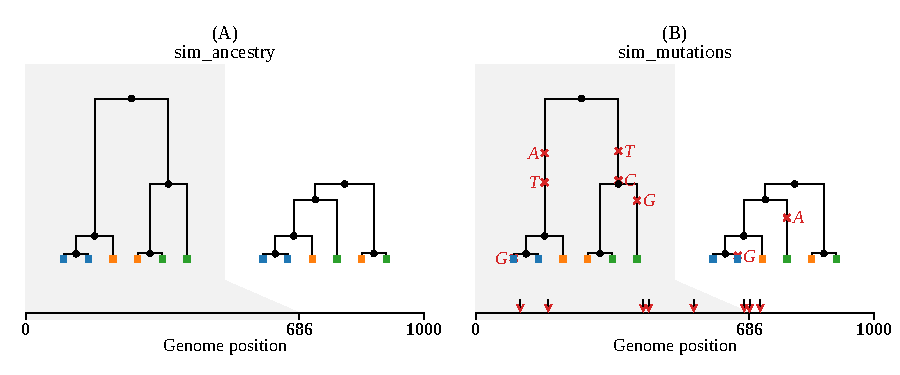
\includegraphics{illustrations/mutated_tree}
    \caption{
        \label{fig-mutated-trees}
        Visualisation of the separation between ancestry and mutation
        simulation. (A) The result of an invocation of \texttt{sim\_ancestry}
        is two trees along a 1kb chunk of genome relating three diploid samples.
        Each diploid individual consists of two genomes (or nodes), indicated
        by colour.
        (B) This ancestry is provided as the input to \texttt{sim\_mutations},
        which adds mutations.
        Graphics produced using \tskit's \texttt{draw\_svg} method.
    }
\end{figure}

A major change for the \msprime\ 1.0 release is the introduction of a new set of APIs,
designed in part to avoid sources of error (see the Demography section) but
also to provide more appropriate defaults while keeping compatibility with
existing code. In the new APIs, ancestry and mutation simulation are fully
separated (see Fig.~\ref{fig-mutated-trees}),
with the \texttt{sim\_ancestry} and \texttt{sim\_mutations}
functions replacing the legacy \texttt{simulate} function. Among other changes,
the new APIs default to discrete genome coordinates and finite sites mutations,
making the default settings more realistic and resolving a major source of confusion and error.
The previous APIs are fully
supported and tested, and will be maintained for the foreseeable future.
The \texttt{msp} program has been extended to include new commands
for simulating ancestry and mutations separately. A particularly useful
feature is the ability to specify demographic models in
Demes format~\citep{gower2021demes} from the command line,
making simulation of complex demographies straightforward.
We also provide an \ms\ compatible
command line interface to support existing workflows.

% The data model
\subsection*{Tree sequences}
\label{sec-ts}

\begin{figure}
\begin{center}
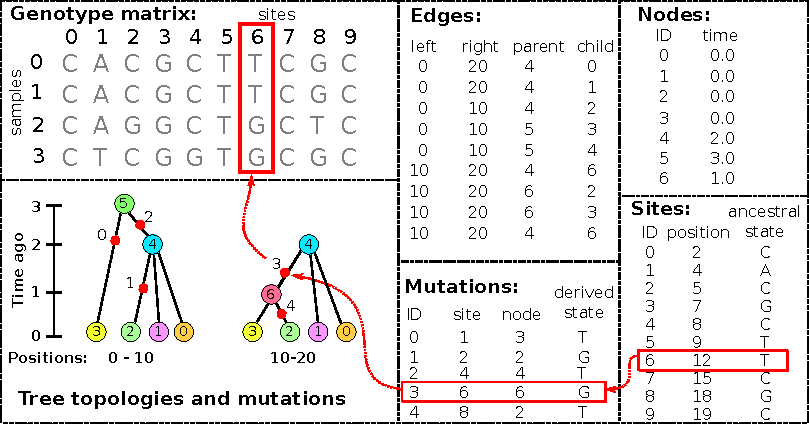
\includegraphics{illustrations/example_tree_sequence}
\end{center}
\caption{\label{fig-ts-example} An example tree sequence describing
genealogies and sequence variation for four samples at ten sites
on a chromosome of twenty bases long.
Information is stored in a set of tables
(the tables shown here include only essential columns, and
much more information can be associated with the various entities).
The node table
stores information about sampled and ancestral genomes. The
edge table describes how these genomes are related along a
chromosome, and defines the marginal trees at each position.
The site and mutation tables together describe sequence variation
% JK: also amongst the ancestral genomes, but only in positions where
% they inherit from the sample. I thought it would be less confusing
% to leave this out?
among the samples.
}
\end{figure}

One of the key reasons for \msprime's substantial performance advantage
over other simulators~\citep{kelleher2016efficient}
is its use of the ``succinct tree sequence''
data structure to represent simulation results.
The succinct tree sequence (usually abbreviated to ``tree sequence'')
was introduced by \cite{kelleher2016efficient}
to concisely encode genetic ancestry and sequence variation
and was originally implemented as part of \msprime.
We subsequently extracted the core tree sequence functionality
from \msprime\ to create the \tskit\ library,
which provides a large suite of tools for processing genetic ancestry
and variation data via APIs
in the Python and C languages~\citep{tskit2021tskit}.
While a full discussion of tree sequences and the capabilities
of \tskit\ is beyond the scope of this article, we summarise
some aspects that are important for simulation.

% Encoding ancestry
% JK: we can say this some other way, this just seemed like the
% most concise way. People may be irritated by being told what
% the definition of a "genome" is, but I think we need to be explicit.
Let us define a genome as the complete set of genetic material
that a child inherits from one parent. Thus, a diploid individual
has two (monoploid) genomes, one inherited from each parent. Since
each diploid individual lies at the end of two distinct lineages
of descent, they will be represented by \emph{two} places (nodes)
in any genealogical tree. In the tree sequence encoding a
\emph{node} therefore corresponds to a single genome, which
is associated with its creation time (and other optional information),
and recorded in a simple tabular format (Fig.~\ref{fig-ts-example}).
Genetic inheritance between genomes (nodes) % delete?
is defined by edges.
An \emph{edge} consists of a
parent node, a child node and the left and right coordinates
% JK: This is potentially confusing. Changed "genomic interval"
% to "chromosome" interval to avoid talking about "the" genome.
of the contiguous chromosomal segment over which
the child genome inherited genetic material from the parent genome.
Parent and child nodes may correspond to ancestor and descendant
genomes separated by many generations.
Critically, edges can span multiple marginal trees along the
genome, and identical node IDs across different trees corresponds
to the same ancestral genome.
For example, in Fig.~\ref{fig-ts-example} the branch from node
0 to 4 is present in both marginal trees, and represented
by a single edge (the first row in the edge table).
This simple device, of explicitly associating tree nodes
with specific ancestral genomes and recording the
contiguous segments over which parent-child relationships exist,
generalises the original
``coalescence records'' concept~\citep{kelleher2016efficient},
and is the key to the efficiency of tree
sequences~\citep{
kelleher2018efficient,kelleher2019inferring,ralph2020efficiently}.
See the \nameref{sec-arg} section below for a discussion of this
closely related concept.

% OK, back to tree sequences: what about sequence variation?
The final output of most population genetic simulations is some representation
of sequence variation among the specified samples. For coalescent
simulations, we usually have three steps: (1) simulate
the genetic ancestry, and optionally output the resulting marginal trees;
(2) simulate sequence evolution conditioned on this ancestry by generating
mutations (see the \nameref{sec-mutations} section); and (3) output the
resulting nucleotide sequences by percolating the effects of the mutations through
the trees. Information about the mutations
themselves---e.g., where they have occurred on the
trees---is usually not retained or made available for subsequent analysis.
In \msprime, however, we skip step (3), instead using \tskit's
combined data model of ancestry and mutations
to represent the simulated sequences.
As illustrated in Fig.~\ref{fig-ts-example}, mutations are a
fully integrated part of \tskit's tree sequence data model, and genetic
variation is encoded by recording sites at which mutations
have occurred, and where each mutation at those sites
has occurred on the marginal tree.
Crucially, the genome sequences themselves are never stored, or indeed directly
represented in memory (although \tskit\ can output the variant matrix
in various formats, if required).
It may at first seem inconvenient to have only this indirect representation
of the genome sequences, but it is extremely powerful.
Firstly, the storage space required for simulations is dramatically
reduced. For a simulation of $n$ samples with $m$ variant sites,
we would require $O(nm)$ space to store the sequence data as a variant
matrix. However, if this simulation was of a recombining genome
with $t$ trees, then the \tskit\ tree sequence encoding
requires $O(n + t + m)$ space,
assuming we have $O(1)$ mutations at each site~\citep{kelleher2016efficient}.
For large sample sizes, this difference is profound, making it
conceivable, for example, to store the genetic ancestry
and variation data for the entire human population on a
laptop~\citep{kelleher2019inferring}. As well as the huge
difference in storage efficiency, it is often far more efficient
to compute statistics of the sequence data from the
trees and mutations than it is to work with the sequences themselves.
For example, computing Tajima's $D$ from simulated data stored in the \tskit\ format
is several orders of magnitude faster than efficient variant matrix
libraries for large sample sizes~\citep{ralph2020efficiently}.

The vast genomic datasets produced during the SARS-CoV-2 pandemic
have highlighted the advantages of storing genetic variation data using the underlying trees.
\cite{turakhia2021ultrafast} propose the
Mutation Annotated Tree (MAT)
format (consisting of a Newick tree
and associated mutations in a binary format) and
the \texttt{matUtils} program as an efficient way to store
and process large viral datasets~\citep{mcbroome2021daily},
achieving excellent compression and processing performance.
Similarly, \phastsim~\citep{demaio2021phastsim}
was developed to simulate sequence evolution on such large SARS-CoV-2
phylogenies, and also outputs a Newick tree annotated with mutations (not
in MAT format) to avoid the bottleneck of generating
and storing the simulated sequences.
While these methods illustrate the advantages of the general
approach of storing ancestry and mutations rather than sequences,
they do not generalise beyond their immediate settings, and
no software library support is available.
% \msprime, on the other hand, provides a fast, powerful, and well-tested
% generic interface for generating and storing mutations on trees.

The software ecosystem built around \tskit\ is stable and mature;
simulators such as
\fwdpy~\citep{thornton2014cpp},
\SLiM~\citep{haller2019slim},
\stdpopsim~\citep{adrion2020community},
\texttt{Geonomics}~\citep{de2021geonomics}
and
\texttt{GSpace}~\citep{virgoulay2021gspace},
and inference methods such as
\texttt{tsinfer}~\citep{kelleher2019inferring},
\texttt{tsdate}~\citep{,wohns2021unified}
and \texttt{Relate}~\citep{speidel2019method}
use either the Python or C
APIs to support outputting results in tree sequence format.
Tree sequences are stored in an efficient binary file format, and
are fully portable across operating systems and processor
architectures. The \tskit\ library ensures interoperability
between programs by having strict definitions of how the
information in each of the tables is interpreted, and
stringent checks for the internal consistency of the data model.

% The output - what do we get out?
\subsection*{Data analysis}
\label{sec-data-analysis}
% We could drop this first sentence?
% The point of running simulations is to generate data, and there
% are two important ways in which the \tskit\ tree sequences output by
% \msprime\ are more useful than classical methods:
% they are more efficient and they contain more information.
% We will consider these points in turn.

The standard way of representing simulation data is
to render the results in a text format, which must subsequently
be parsed and processed as part of some analysis pipeline. For example,
\ms\ outputs a set of sequences
and can also optionally output the marginal trees along
the genome in Newick format,
and variants of this approach are used by many simulators.
Text files have many advantages, but are slow to process at scale.
The ability to efficiently process simulation results is
particularly important in simulation-based inference methods
such as Approximate Bayesian Computation
(ABC)~\citep{beaumont2002approximate,csillery2010approximate,wegmann2010abctoolbox}
and machine learning based
approaches~\citep{sheehan2016deep,chan2018likelihood,schrider2018supervised,
flagel2019unreasonable,sanchez2020deep}. Clearly, simulation efficiency is
crucial since the size and number of simulations that can be performed determines
the depth to which one can sample from the model and parameter space.
Equally important,
however, is the efficiency with which the simulation results can be
transformed into the specific input required by the inference method.
In the case of ABC, this is usually a set of summary statistics of the sequence
data, and methods avoid the bottleneck of parsing
text-based file formats to compute these statistics
by either developing their own
simulators~\citep[e.g.][]{cornuet2008inferring,lopes2009popabc}
or creating forked versions (i.e., modified copies) of existing
simulators~\cite[e.g.][]{thornton2006approximate,
hickerson2007msbayes,pavlidis2010msabc,huang2011mtml,quinto2018modeling},
tightly integrated with the inference method.
Modern approaches to ABC such as
ABC-RF~\citep{raynal2019abc,pudlo2016abc} and
ABC-NN~\citep{csillery2012abc,blum2010abc} use large
numbers of weakly informative statistics,
making the need to efficiently compute statistics from simulation
results all the more acute.
By using the stable APIs and efficient data interchange mechanisms
provided by \tskit,
the results of an \msprime\ simulation can be immediately processed,
without format conversion overhead.
The \tskit\ library has a rich suite of population
genetic statistics and other utilities, and is in many cases
orders of magnitude faster than matrix-based methods for
large sample sizes~\citep{ralph2020efficiently}. Thus, the combination
of \msprime\ and \tskit\ substantially increases the overall
efficiency of many simulation analysis pipelines.

Classical text based output formats like \ms\ are inefficient to process,
but also lack a great deal of important information about the simulated
process.
The tree-by-tree topology information output by simulators in Newick
format lacks any concept of node identity,
and means that we cannot reliably infer information about ancestors
from the output. Because Newick stores branch lengths rather
than node times, numerical precision issues also arise for
large trees~\citep{mcgill2013graphml}.
Numerous forks  of simulators have been created to access information not provided
in the output. For example, \ms\  has been forked to
output information about migrating segments~\citep{rosenzweig2016powerful},
ancestral lineages~\citep{chen2013asymptotic},
% leaving this out because it's not about hidden information
% an array of population genetic statistics~\citep{ramos2007mlcoalsim}
% Any more?
and \ms's fork \msHOT~\citep{hellenthal2007mshot}
has in turn been forked to output information on local
ancestry~\citep{racimo2017archaic}.
All of this information
is either directly available by default in \msprime, or can be optionally
stored via options such as \texttt{record\_migrations} or
\texttt{record\_full\_arg} (see the \nameref{sec-arg} section) and
can be efficiently and conveniently processed via \tskit\ APIs.

% These problems of inefficient and limited access to the simulated
% data are comprehensively solved by \msprime\ and \tskit. Complete
% information about ancestry and mutation in simulations is immediately
% available to the user in a single integrated data structure
% (rather than multiple independent files), with no intermediate
% processing required.
% Users can subsequently compute precisely the information that they
% require using the powerful suite of population genetic statistics
% and other methods available in \tskit.

% Stuff we simulate: mutations
\subsection*{Simulating mutations}
\label{sec-mutations}

% Explain the background: what have people done classically?
Because coalescent simulations are usually concerned with
neutral evolution (see the \nameref{sec-selection} section, however)
the problem of generating synthetic genetic variation can be decomposed into
two independent steps:
firstly, simulating genetic ancestry (the trees), then subsequently simulating
variation by superimposing mutation processes on those trees
(see Fig.~\ref{fig-mutated-trees}).
A number of programs exist to place mutations on trees: for instance,
the classical \SeqGen\ program~\citep{rambaut1997seq}
supports a range of different models of sequence evolution,
and various extensions to the basic
models have been proposed~\citep[e.g.][]{cartwright2005dna,fletcher2009indelible}.
Partly for efficiency and partly in the interest of
simplicity for users (i.e., to avoid intermediate text format conversions),
population genetic simulators have tended to
include their own implementations of mutation simulation, with
most supporting the infinite sites
model~\citep[e.g.][]{hudson2002generating}
but with several supporting a wide range of different models of sequence
evolution~\citep[e.g.][]{mailund2005coasim,excoffier2011fastsimcoal,
virgoulay2021gspace}. Thus, despite the logical separation between
the tasks of simulating ancestry and neutral sequence evolution,
the two have been conflated in practice.

Part of the reason for this poor record of software reuse and modularity is the
lack of standardised file formats, and in particular, the absence of common
library infrastructure to abstract the details of interchanging simulation
data. Although \msprime\ also supports simulating both ancestry and mutations,
the two aspects are functionally independent within the software; both ancestry and mutation simulators are present in \msprime\
for reasons of convenience and history,
and could be split into separate packages.
The efficient C and Python interfaces for
\tskit\ make it straightforward to add further information to
an existing file, and because of its efficient data interchange mechanisms,
there is no performance penalty for additional operations
in a different software package.
Thanks to this interoperability, \msprime's
mutation generator can work with \emph{any} \tskit\ tree sequence,
be it simulated using \SLiM~\citep{haller2019slim} or
\fwdpy~\citep{thornton2014cpp}, or estimated from real
data~\citep{kelleher2019inferring,speidel2019method,wohns2021unified}.
It is a modular
component intended to fit into a larger software ecosystem, and
is in no way dependent on \msprime's ancestry simulator.

As well as providing a new API
that emphasises the logical split between ancestry and mutation simulation,
we have greatly extended the sophistication of
\msprime's mutation generation engine for version 1.0,
achieving near feature-parity with \SeqGen.
We support a large number of mutation models, including the
JC69~\citep{jukes1969evolution},
F84~\citep{felsenstein1996hidden},
and GTR~\citep{tavare1986some} nucleotide models
and the BLOSUM62~\citep{henikoff1992amino}
and PAM~\citep{dayhoff1978} amino acid models.
Other models, such as the Kimura two and three
parameter models~\citep{kimura1980simple,kimura1981estimation},
can be defined easily and efficiently in
user code by specifying a transition matrix between
any number of alleles (which can be arbitrary unicode strings).
Mutation rates can vary along the genome, and multiple mutation
models can be imposed on a tree sequence by overlaying mutations
in multiple passes.
We have extensively validated the results of mutation simulations
against both theoretical expectations and output from
\SeqGen~\citep{rambaut1997seq} and
\Pyvolve~\citep{spielman2015pyvolve}.

\begin{figure}
    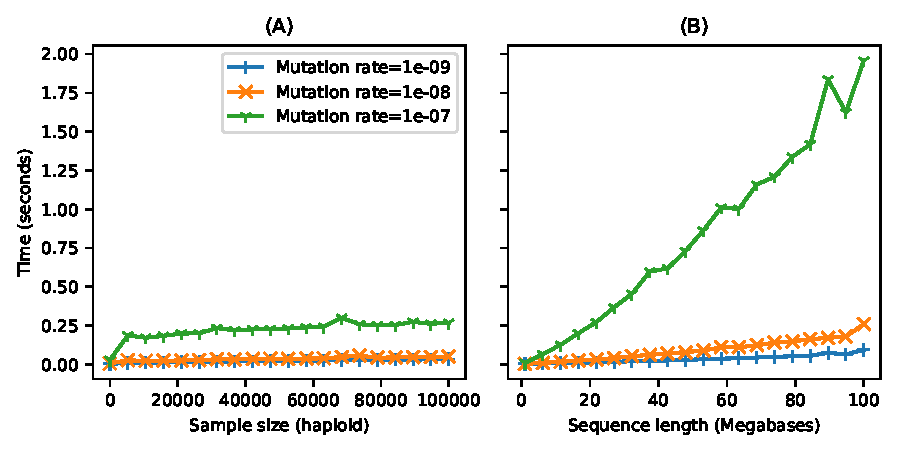
\includegraphics{figures/mutations-perf}
\caption{\label{fig-mutations-perf} Time required to run
\texttt{sim\_mutations} on tree sequences generated
by \texttt{sim\_ancestry} (with a population size of $10^4$
and recombination rate of $10^{-8}$) for varying (haploid) sample
size and sequence length. We ran 10 replicate mutation simulations
each for three different mutation rates, and report the average
CPU time required (Intel Core i7-9700).
(A) Holding sequence length fixed at 10 megabases and varying the
number of samples (tree tips) from 10 to 100,000.
(B) Holding number of samples fixed at 1000, and varying the sequence
length from 1 to 100 megabases.}
\end{figure}

Simulating mutations in \msprime\ is efficient.
Fig.~\ref{fig-mutations-perf} shows the time required to generate
mutations (using the default JC69 model) on
simulated tree sequences for a variety of mutation
rates as we vary the number of samples
(Fig.~\ref{fig-mutations-perf}A) and the sequence
length (Fig.~\ref{fig-mutations-perf}B).
For example, the longest running simulation in
Fig.~\ref{fig-mutations-perf}B required less than 2 seconds to
generate an average of 1.5 million mutations over 137,081 trees
in a tree sequence with 508,125 edges.
This efficiency for large numbers of trees is possible because
the tree sequence encoding allows us to generate mutations
on an edge-by-edge basis
(see Fig.~\ref{fig-ts-example} and the~\nameref{app-mutation-algorithm}
appendix),
rather than tree-by-tree and branch-by-branch as would otherwise be required.
In the above example from Fig.~\ref{fig-mutations-perf}B,
if we generated mutations tree-by-tree, we would have to iterate over 273,887,838 branches
(since there are 137,081 trees and 1,998 branches in each
tree) rather than 508,125 edges, resulting in $\sim$500 times more work.
% python3 evaluation/generate_mutations_perf_data.py benchmark-single-tree
Even if we have a tree sequence consisting of a single tree
(negating the advantage of working edge-by-edge),
\msprime's mutation generator is still very efficient.
For example, we simulated mutations under the BLOSUM62 amino
acid model for a tree with $10^6$ leaves over $10^4$ sites (resulting
in $\sim$260,000 mutations) in about $0.8$ seconds, including
the time required for file input and output.
We do not attempt a systematic benchmarking of \msprime's
mutation generation code against other methods, because at this scale it is
difficult to disentangle the effects of inefficient input and
output formats from the mutation generation algorithms.
Given these timings, it seems unlikely
that generating mutations with \msprime\ would be a bottleneck in any
realistic analysis.

There are many ways in which the mutation generation code
in \msprime\ could be extended. For example, we intend to add support for
microsatellites~\citep{mailund2005coasim},
codon models~\citep{arenas2007recodon}
and indels~\citep{cartwright2005dna,fletcher2009indelible},
although changes may be required to \tskit's data model
which is currently based on the assumption of independent sites.

\subsection*{Recombination}
\label{sec-recombination}

Crossover recombination is implemented in \msprime\ using Hudson's algorithm, which
works backwards in time, generating common ancestor and recombination
events and tracking their effects on segments of ancestral
material inherited from the
sample~\citep{hudson1983properties,hudson1990gene,kelleher2016efficient}.
Common ancestor events merge the ancestral material of two lineages,
and result in coalescences in the marginal trees when ancestral
segments overlap.
Recombination events split the ancestral material for some lineage
at a breakpoint, creating two independent
lineages. Using the appropriate data structures~\citep{kelleher2016efficient},
this process is much more efficient to simulate
than the equivalent left-to-right
approach~\citep{wiuf1999recombination,wiuf1999ancestry}.
In \msprime\ 1.0, recombination rates can vary along a chromosome, allowing
us to simulate recombination hotspots and patterns
of recombination from empirical maps.
The implementation of recombination in \msprime\ is extensively validated
against analytical results~\citep{hudson1983properties,kaplan1985use}
and simulations by \ms, \msHOT\ and \SLiM.

The Sequentially Markovian Coalescent (SMC) is an approximation of the
coalescent with recombination~\citep{mcvean2005approximating,marjoram2006fast},
and was primarily motivated by the need to
simulate longer genomes than was possible using tools like \ms.
The SMC is a good approximation to the
coalescent with recombination when we have fewer than five sampled
genomes~\citep{hobolth2014markovian,wilton2015smc}, but the
effects of the approximation are less well understood for larger
sample sizes, and several approaches have been proposed
that allow simulations to more closely approximate the coalescent
with recombination~\citep{chen2009fast,wang2014new,staab2015scrm}.
The SMC and SMC' models are supported
in \msprime\ 1.0. However, they are currently implemented using a
naive rejection sampling approach, and are somewhat slower
to simulate than the exact coalescent with recombination. These
models are therefore currently only appropriate for studying the
SMC approximations themselves, although we intend to
implement them more efficiently in future versions.

\begin{figure}
\begin{center}
    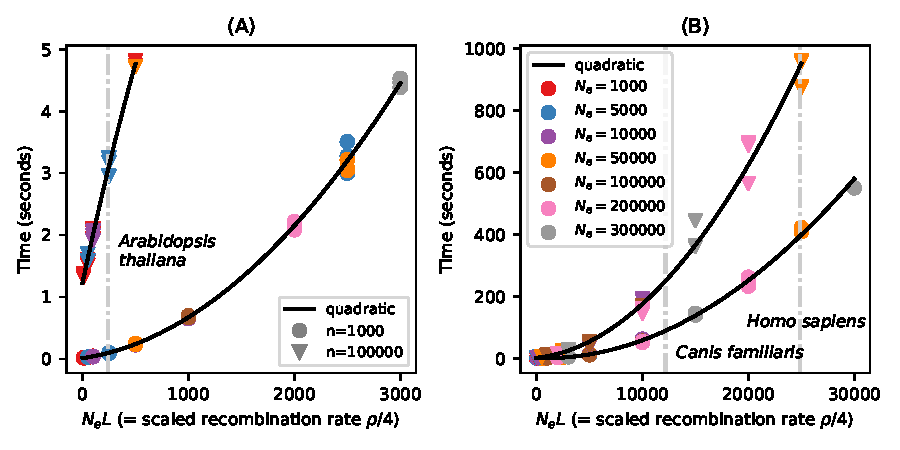
\includegraphics{figures/ancestry-perf}
\end{center}
\caption{\label{fig-ancestry-perf}
    Running time for \msprime\
    for (A) small and (B) larger simulations on an Intel i7-6600U CPU.
    Each point is the run time of one simulation,
    for various values of effective population size ($N_e$),
    chromosome length in Morgans ($L$), and number of samples ($n$).
    Run time scales quadratically with the product of $N_e$ and $L$,
    shown on the horizontal axis. For example, (A) shows that
    1,000 samples of 1 Morgan-length chromosomes
    from a population of $N_e=2,000$ diploids
    would take about 2 seconds, and (equivalently) that the same number of
    0.01 Morgan segments with $N_e=200,000$ would take the same time.
    Since recombination rate in these simulations was $10^{-8}$,
    $L$ is the number of base pairs divided by $10^8$.
    The black lines are quadratic fits separately in each panel
    and sample size. Vertical grey lines show the approximate values of
    $N_e L$ for chromosome 1 in three species, using values from
    the \stdpopsim\ catalogue~\citep{adrion2020community}.
}
\end{figure}

% Output from  python3 evaluation/plot.py ancestry-perf
% Predicted time for DroMel chr2L with n = 1000 = 107.85106995938845 hours
% Predicted time for DroMel chr2L with n = 100000 = -511.74273443828514 hours
% Predicted time for DroMel chr2L with n = 1000 = 177.40184421122058 hours
% Predicted time for DroMel chr2L with n = 100000 = 361.90415260982536 hours

In human-like parameter regimes and for large sample sizes,
\msprime's implementation of the
exact coalescent with recombination comprehensively outperforms
all other simulators, including those based on SMC
approximations~\citep{kelleher2016efficient}. However, it is important
to note that although the implementation of Hudson's algorithm is
very efficient, it is still quadratic in the population scaled recombination rate
$\rho = 4 N_e L$, where $L$ is the length of the genome in units of recombination distance.
This is because Hudson's algorithm tracks recombinations not only
in segments ancestral to the sample, but also between ancestral segments.
As mentioned above, common ancestor events in which the ancestral material
of two lineages is merged only result in coalescences in the marginal trees
if their ancestral segments overlap. If there is no overlap, the merged
segments represent an ancestral chromosome that is a genetic ancestor
of the two lineages, but not the most recent common genetic ancestor
at any location along the genome.
When this happens, the merged lineage carries ``trapped'' genetic material
that is not ancestral to any samples, but where recombinations can still occur.
The SMC approximations work by disallowing common ancestor events
that generate trapped material, greatly simplifying the process.
However, this also removes subtle long-range
correlations in the trees since there are many ways in which ancestry
segments can merge without overlapping.

For large $\rho$, recombination events in trapped ancestral material will
dominate, and so we can use this as a proxy for the overall number
of events in Hudson's algorithm.
\citet[Eq.~5.10]{hein2004gene} gave
\begin{equation}\label{eqn-hsw-bound}
\rho (\rho + 1) \left( \sum_{i=1}^{n-1} \frac{1}{i} \right)^2
\end{equation}
as an upper bound
on the number of recombination events within trapped ancestral material
in Hudson's algorithm for $n$ samples.
% Since the sum is well approximated by $\log{n}$,
% a natural conjecture is that the time complexity of Hudson's
% algorithm is $O(\rho^2 \log^2 n)$.
Fig.~\ref{fig-ancestry-perf} shows the observed run time for
simulations with a variety of population size, chromosome
length and sample sizes, and demonstrates that Eq.~\eqref{eqn-hsw-bound}
correctly predicts the quadratic dependence on $\rho$,
as previously conjectured~\citep[Fig.~2]{kelleher2016efficient}.
We also see that the dependence on $n$ is quite weak,
since increasing sample size 100-fold
only increases run time by a factor of 2 or so. However, the
$\log^2{n}$ factor implied by Eq.~\eqref{eqn-hsw-bound}
(the sum is a harmonic number and can be approximated by $\log{n}$)
is not well supported by observed run times (or numbers of events)
except possibly at very
large values of $\rho$. It therefore appears that a different dependence
on $n$ is required to accurately predict simulation time for a
given $\rho$ and $n$.

Fig.~\ref{fig-ancestry-perf} is a useful yardstick, allowing us
to predict how long simulations should take for a wide range of
species. Taking a typical chromosome to be 1 Morgan in length,
these plots show, roughly, that simulating chromosome-length
samples from a population of thousands of individuals takes seconds,
while samples from a population of tens of thousands take minutes.
Simulating whole chromosomes for many species is very fast,
with 1000 samples of chromosome 1 for
\emph{Arabidopsis thaliana} taking less than a second, and a few
minutes for dogs and humans. However, the dependence on $\rho$
\emph{is} quadratic, and if $\rho$ is sufficiently large simulations
may not be feasible. For example,
the \emph{Drosophila melanogaster} chromosome 2L
is about 23.5Mb long with an average recombination rate of around $2.4 \times 10^{-8}$,
so $L \approx 0.57$,
and with $N_e = 1.7 \times 10^6$ \citep{li2006inferring},
$N_e L \approx 10^6$, so extrapolating the curve in Fig.~\ref{fig-ancestry-perf}B
predicts that simulation would require around 177 hours for 1000 samples.
For such large values of $\rho$  we recommend
users consider approximate simulations. Since \msprime\ does not currently
have efficient implementations of approximate coalescent with recombination
models, in these cases we recommend using SMC based methods such as \scrm,
particularly if sample sizes are small.
In practice, to predict the running time of a given
simulation in \msprime, we recommend that users
measure run time in a series of simulations with short genome lengths and
the desired sample size,
and then predict run time by fitting a quadratic curve to genome length
as in Fig.~\ref{fig-ancestry-perf}.
It is important to note that the quadratic curves in the two
panels of Fig.~\ref{fig-ancestry-perf} are different, and
predicting the run times of days-long simulations
using the timing of seconds-long runs is unlikely to be very accurate.

What about simulations with changing population size?
To understand how run time depends on demography
it helps to consider why run time is quadratic in $\rho$.
At any point in time, \msprime\ must keep track of some number of lineages,
each of which contains some number of chunks of genetic material.
Common ancestor events reduce the number of lineages,
and recombination events increase their number.
However, with long genomes,
only a small fraction of the common ancestor events
will involve overlapping segments of ancestry
and lead to coalescence in the marginal trees.
Such disjoint segments are often far apart (on average, about distance $L/2$),
and so recombine apart again immediately;
it is these large numbers of rapid and inconsequential events that
lead to the quadratic run time.
The maximum number of lineages occurs when
the increase and decrease in numbers of lineages due to
common ancestor and recombination events balance out.
To get an idea of run time we can estimate when this balance occurs.
Suppose that the maximum number of lineages is $M$;
at this time the rate of common ancestor events is $M (M-1) / (4 N_e)$
and the total rate of recombination is $M \ell$,
where $\ell$ is the mean length of genome carried by each lineage
(including ``trapped'' non-ancestral material).
At the maximum, coalescence and recombination rates are equal,
so a typical segment of ancestry will spend roughly half its time
in a lineage with at least one other such segment---and,
since such lineages carry at least two segments,
at most one-third of the lineages carry long trapped segments of ancestry.
Since the maximum number of lineages is reached
very quickly~\citep{nelson2020accounting},
this implies that $\ell \approx L / 6$.
Setting the rates of recombination and common ancestor events
to be equal and solving for $M$,
we find that $M$ is roughly equal to $L N_e$.
The number of lineages then decreases gradually from this maximum
on the coalescent time scale, and therefore over roughly $2 N_e$ generations.
Since the total rate of events when the maximum number of lineages is
present is roughly $L^2 N_e / 6$,
then the total number of events is proportional to $(L N_e)^2$---i.e.,
proportional to $\rho^2$.

What does this tell us about run time for simulating time-varying population sizes?
The argument above implies that the work is spread out relatively
evenly on the coalescent time scale.
Suppose that population size today is $N_1$,
while $T$ generations ago it was $N_2$.
Does the run time depend more on $4 N_1 L$ or $4 N_2 L$?
The answer depends on how $T$ compares to $N_1$: if $T/N_1$ is large,
then run time will be similar to a population of size $N_1$;
while if $T/N_1$ is small, it will be similar to a population of size $N_2$.
For instance, in many agricultural species $N_1 \propto 100$, while $N_2 \propto 10^5$,
and the run time will depend critically on $T$---in other words,
simulation will be quick in a species with a strong domestication bottleneck,
and slow otherwise.

\subsection*{Gene conversion}
Gene conversion is a form of recombination that results in the transfer
of a short segment of genetic material,
for example between homologous chromosomes~\citep{chen2007gene}.
Since gene conversion impacts much shorter segments than
crossover recombination (typically below 1kb) it
affects patterns of linkage disequilibrium differently~\citep{korunes2017gene}.
\cite{wiuf2000coalescent} modelled gene conversion in the coalescent
via a rate at which gene conversion events are initiated
along the genome and a geometrically distributed tract length.
In terms of the ancestral process, gene conversion differs from
crossover recombination (as described in the previous section)
in that it extracts a short tract of ancestry into
an independent lineage, rather than splitting ancestry
to the left and right of a given breakpoint.
We have implemented this model of gene
conversion in \msprime\ 1.0, and validated the output against
\ms\ and analytical results~\citep{wiuf2000coalescent}.

\begin{figure}
\begin{center}
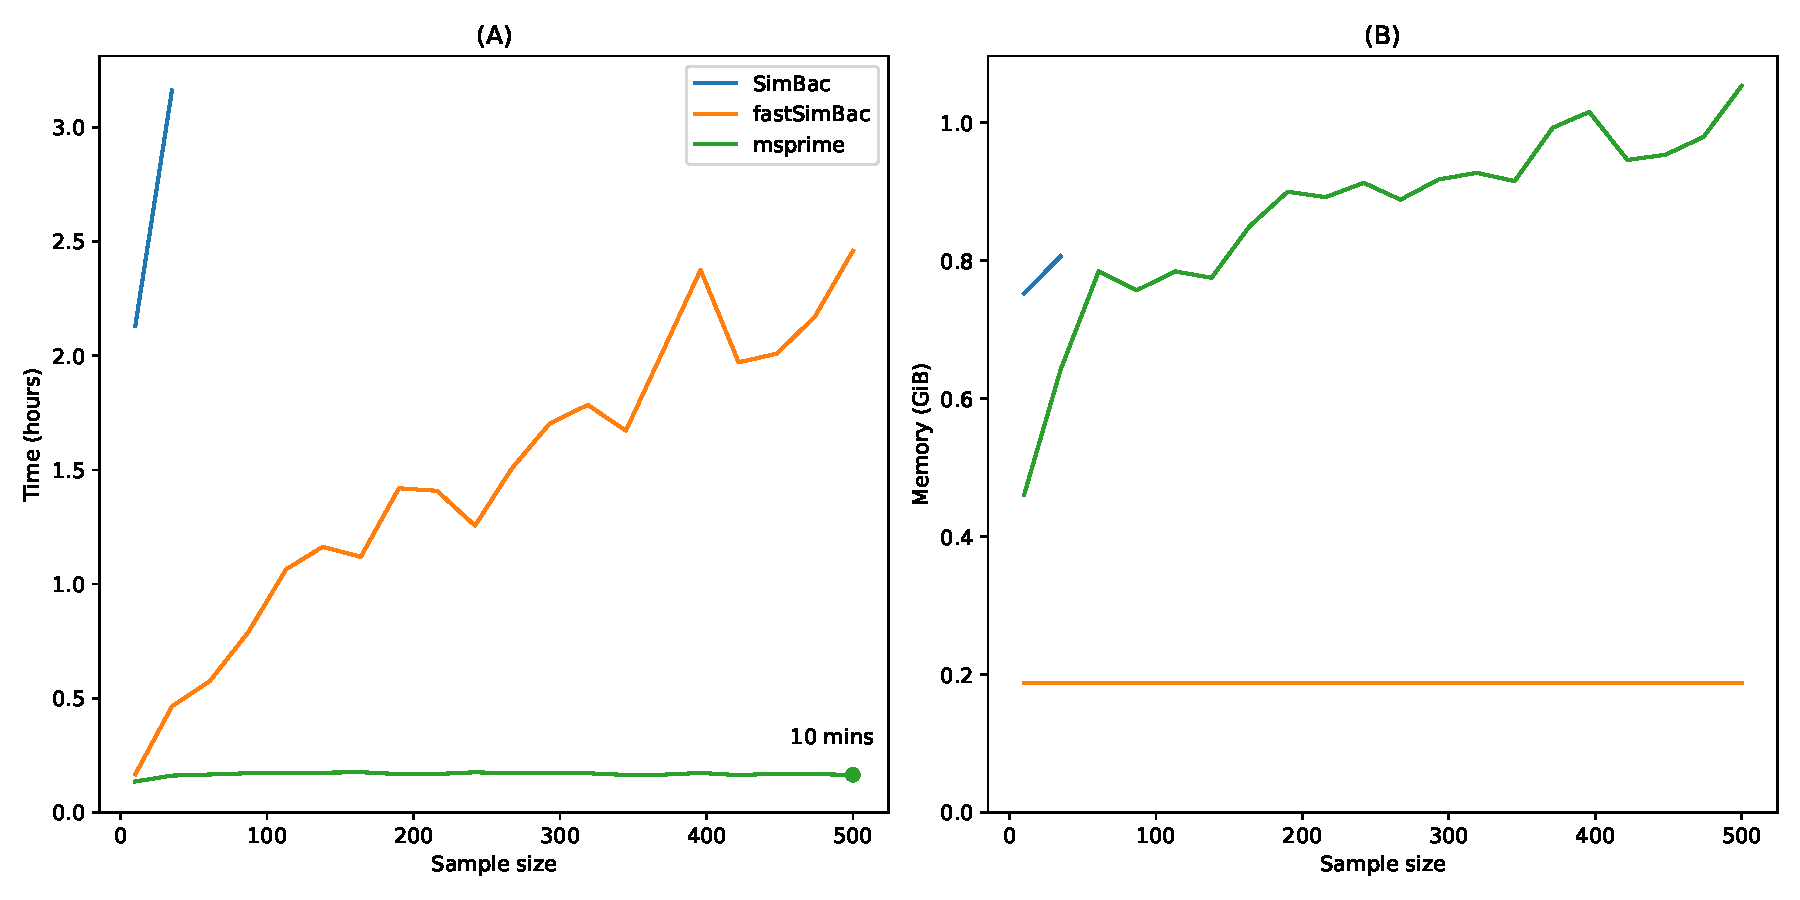
\includegraphics{figures/gc-perf}
\end{center}
\caption{\label{fig-gc-perf}Comparison of simulation performance
using \msprime, \SimBac, and \FastSimBac\ for varying sample sizes,
with parameters roughly equivalent to the current estimate
for \textit{E.~coli}~\citep{lapierre2016the}:
a 4.5Mb genome with scaled gene conversion rate of 0.015 and
a mean tract length of 500.
We report (A) the total CPU time and (B) maximum memory usage
averaged over 5 replicates (Intel Xeon E5-2680 CPU).
We did not run \SimBac\ beyond first two data points because
of the very long running times.}
% The genome length was set to 4.5 Mb, the scaled per site
% gene conversion rate was set to $N_e g = \gamma = 0.015$ and
% the mean gene conversion tract length was set to $L = 500$, which is close to
% estimated parameters for \textit{E.~coli}, i.e.\ an effective populations size
% $N_e = 1.8e^8$ and a per site per generation conversion rate $g = 8.9e^{-11}$
% with mean tract length $L = 542$~\citep{lapierre2016the}.}
\end{figure}

Gene conversion is particularly useful to model homologous recombination in
bacterial evolution,
and so we compare the performance of \msprime\ with gene conversion to
two specialised bacterial simulators,
\SimBac~\citep{brown2016simbac} and \FastSimBac~\citep{demaio2017the}.
Figure~\ref{fig-gc-perf}A shows that \msprime\ is far more efficient than
both \SimBac\ and the SMC-based approximation \FastSimBac.
Figure~\ref{fig-gc-perf}B shows that \msprime\ requires somewhat more memory
than \FastSimBac, (as expected since \FastSimBac\ uses a left-to-right
SMC approximation) but is still reasonably modest at around 1GiB for a simulation
of 500 whole \emph{E.~coli} genomes.
However, \msprime\ is currently lacking many of the specialised features
required to model bacteria, and so an important avenue for future work
is to add features such as circular genomes
and bacterial gene transfer~\citep{baumdicker2014AGTG}.

In terms of predicting the run time for a simulation including gene conversion,
we recommend following the same approach as discussed in the previous section:
run a number of simulations for short genome lengths, fit a quadratic to the
observed CPU times, and use this to predict run time for larger simulations.
Depending on the relative contributions of gene conversion and crossover
recombination, this may be an over-estimate since gene conversion events
tend to generate less trapped ancestral material than crossovers.
Thus, simulations using mammalian-like gene conversion parameters
may run faster than simulations in which an equivalent amount of
crossover recombination is imposed.
% TODO check this again!
Since each gene conversion creates two breakpoints and a crossover
creates only one, we expect the output tree sequence for a given rate
of gene conversion to be roughly twice the size of the output from a simulation
with the same rate of crossovers.

\subsection*{Demography}
\label{sec-demography}
% TODO should we put in some citations here for the models? Hardly seems
% necessary.
One of the key applications of population genetic simulations is to generate
data for complex demographies. Beyond idealised cases such as stepping-stone or
island models, or specialised cases such as isolation-with-migration models,
analytical results are rarely possible. Simulation is therefore integral to the
development and evaluation of methods for demographic inference. The demography
model in \msprime\ is directly derived from the approach used in \ms, and
supports an arbitrary number of randomly mating populations exchanging migrants
at specified rates. A range of demographic events are supported, which allow for
varying population sizes and growth rates, changing migration rates over time,
as well as population splits, admixtures and pulse migrations.
The location of sampled lineages
can be tracked through time in as much detail as required: each tree node is
automatically associated with the population in which it arose, the location of
lineages can be recorded at any given time via census events, or every lineage
migration can be recorded.
Large demographic models can be simulated efficiently in version \msprime\ 1.0,
since we only consider populations that contain lineages and
have non-zero migration rates when generating migration event
waiting times. This is a considerable improvement
over version 0.x, which scaled quadratically with the number of populations.

A major change for \msprime\ 1.0 is the introduction of the new Demography API,
designed to address a design flaw in the \msprime\ 0.x interface which led to
a number of avoidable errors in downstream
simulations~\citep{ragsdale2020lessons}. Briefly, the 0.x API required three
separate parameters be provided to the \texttt{simulate} function to describe a
demographic model, making it easy to accidentally omit information. The 1.0 API
resolves this issue by creating a new \texttt{Demography} class, which
encapsulates all information about the demographic model, and fully decouples
the definition from other simulation details. An instance of this class is then
provided as a parameter to the new \texttt{sim\_ancestry} function,
substantially reducing the potential for error.
Another improvement over the
0.x APIs is the introduction of explicit population split and admixture events,
and a population state machine that ensures that lineages cannot migrate into
(or be sampled from) inactive populations. This demography model is compatible
with the Demes standard~\citep{gower2021demes}, and the \texttt{Demography}
class supports importing and exporting Demes models.
Models previously constructed using the 0.x API can be seamlessly imported into
the \texttt{Demography} class, and we also support importing demographic
models from Newick species trees and the output of programs
like *BEAST~\citep{heled2009bayesian}.

The \texttt{DemographyDebugger} provides detailed information about
demographic models as well as numerical methods to make predictions
about these models. For example, we can compute
the coalescence rates for two or more lineages
drawn from populations at specified times in the past,
which can inverted to obtain the
``inverse instantaneous coalescence rate'' of \citet{chikhi2018iicr}.
Many popular approaches in population genetics use the distribution of
coalescence rates between pairs of lineages in one or more populations to infer
effective population sizes over
time~\citep{li2011inference,sheehan2013estimating,schiffels2014inferring} or
split times and subsequent migration rates between
populations~\citep{wang2020tracking}.
These numerical methods provide a valuable
ground-truth when evaluating such inference methods, as illustrated by
\cite{adrion2020community}.

\subsection*{Instantaneous bottlenecks}

A common approach to modelling the effect of demographic history on genealogies
is to assume that effective population size ($N_e$) changes in discrete steps
which define a series of epochs~\citep{griffiths1994sampling, marth2004allele,
keightley2007joint,li2011inference}. In this setting of piecewise constant
$N_e$, capturing a population bottleneck requires three epochs: $N_e$ is
reduced by some fraction $b$ at the start of the bottleneck, $T_{start}$, and
recovers to its initial value at time $T_{end}$~\citep{marth2004allele}. If
bottlenecks are short both on the timescale of coalescence and mutations,
there may be little information about the duration of a bottleneck
($T_{end}-T_{start}$) in sequence data. Thus a simpler, alternative model is to
assume that bottlenecks are instantaneous ($T_{end}-T_{start} \rightarrow 0$)
and generate a sudden burst of coalescence events (a multiple merger event) in
the genealogy. The strength of the bottleneck $B$ can be thought of as an
(imaginary) time period during which coalescence events are collapsed,
i.e.\ there is no growth in genealogical branches during $B$ and the probability that a
single pair of lineages entering the bottleneck coalesce during the bottleneck
is $1-e^{-B}$. Although this simple two parameter model of bottlenecks is
attractive and both analytic results and empirical
inference~\citep{griffiths1994sampling, galtier2000detecting,
bunnefeld2015inferring} have been developed under this model, there has
been no software available to simulate data under instantaneous
bottleneck histories.

We have implemented instantaneous bottlenecks in \msprime~1.0
using a variant of Hudson's linear time single-locus coalescent
algorithm~\citep{hudson1990gene}. Instantaneous bottlenecks are specified
by adding events to the \texttt{Demography} class
(see the \nameref{sec-demography} section)
and can be used in combination with any other demographic modelling
features. We have validated the results of these simulations by comparing
against analytical expectations for coalescence times and the
site frequency spectrum~\citep{bunnefeld2015inferring}.

\subsection*{Multiple merger coalescents}

Kingman's coalescent assumes that only two ancestral lineages can merge at
each merger event. Although this is generally a reasonable approximation, there
are certain situations in which the underlying mathematical assumptions are
violated. For example in certain highly fecund organisms
\citep{hedgecock_94,B94,HP11,A04,irwin16}, where individuals have the ability
to produce numbers of offspring on the order of the population size and
therefore a few individuals may produce the bulk of the offspring in any given
generation~\citep{hedgecock_94}. These population dynamics violate basic
assumptions of the Kingman coalescent, and are better modelled by
`multiple-merger' coalescents \citep{DK99,P99,S99,S00,MS01}, in which more than
two lineages can merge in a given event. Multiple-merger coalescent processes
have also been shown to be relevant for modelling the effects of selection on
gene genealogies
\citep{Gillespie909,DS04,desai2013genetic,neher2013genealogies,schweinsberg2017rigorous}.

Although multiple merger coalescents have been of significant theoretical
interest for around two decades, there has been little practical software
available to simulate these models.
\cite{kelleher2013coalescent,kelleher2014coalescent} developed packages to
simulate a related spatial continuum model~\citep{barton2010new},
\cite{zhu2015hybrid} simulate genealogies within a species tree
based on a multiple-merger model, and
\cite{becheler2020occupancy} provide a general method for simulating
multiple merger processes
as part of the Quetzal framework~\citep{becheler2019quetzal}.
The \texttt{Beta-Xi-Sim} simulator~\citep{koskela2018multi,koskela2019robust}
also includes a number of extensions to the Beta-coalescent.
None of these methods work with large genomes, and very little work
has been performed on simulating multiple merger processes with recombination.

We have added two multiple merger coalescent models in \msprime\ 1.0, the
Beta-coalescent~\citep{schweinsberg03} and
``Dirac''-coalescent~\citep{BBE13}, allowing us to efficiently simulate
such models with recombination for the first time.
These simulation models have been extensively validated against
analytical results from the site frequency
spectrum~\citep{birkner2013statistical,blath2016site,hobolth2019phase}
 as well as more general properties of coalescent processes.
See the Appendix for more details and model derivations.

\subsection*{Ancestral Recombination Graphs}
\label{sec-arg}

The Ancestral Recombination Graph (ARG) was introduced by
Griffiths~\citep{griffiths1991two,griffiths1997ancestral}
as a representation of the coalescent with recombination
stochastic process as a graph.
This formulation is complementary to Hudson's earlier
work~\citep{hudson1983properties}, and substantially increased our theoretical
understanding of recombination. In Griffiths' ARG formulation,
a realisation of the coalescent with recombination is a graph in which
vertices represent common ancestor or recombination events, and edges represent
lineages. There is the ``big'' ARG, in which we track lineages arising out of
recombinations regardless of whether they carry ancestral
material~\citep{ethier1990two},
% and
% consequently wait an exponentially large time until all sampled lineages
% coalesce into a single ancestor~\citep{ethier1990two},
and the ``little'' ARG in which we only track genetic ancestors.
Over time, usage of the term
has shifted away from its original definition as a stochastic process,
to being interpreted as a representation of a particular genetic ancestry
as a graph, without necessarily following the specific details of the Griffiths
formulation~\citep[e.g.][]{minichiello2006mapping,mathieson2020ancestry}.
Under the latter interpretation,
the tree sequence encoding of genetic ancestry (described above)
clearly \emph{is} an ARG: the nodes and edges
define a graph in which edges are annotated with the
set of disjoint genomic intervals
through which ancestry flows.

\begin{figure}
\begin{subfigure}[t]{0.33\textwidth}
\centering
\caption*{(A)}
    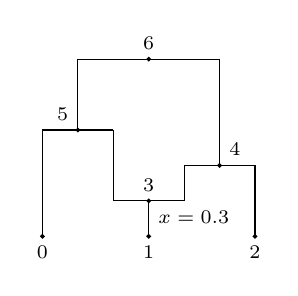
\begin{tikzpicture}[scale=0.45,nodestyle/.style={font=\scriptsize}]

    \draw (-2,0) -- (-2,3) -- (0, 3);
    \draw (1,0) -- (1,1);
    \draw (0,1) -- (2,1) -- (2,2) -- (4,2) -- (4,0);
    \draw (3,2) -- (3,5);
    \draw (0,1) -- (0,3);
    \draw (-1, 3) -- (-1, 5) -- (3,5);

    \draw[fill] (-2,0) circle [radius=0.05];
    \draw[fill] (-1,3) circle [radius=0.05];
    \draw[fill] (1,0) circle [radius=0.05];
    \draw[fill] (4,0) circle [radius=0.05];
    \draw[fill] (1,1) circle [radius=0.05];
    \draw[fill] (3,2) circle [radius=0.05];
    \draw[fill] (1,5) circle [radius=0.05];

    \node[nodestyle] [below] at (-2,0) {0};
    \node[nodestyle] [below] at (1,0) {1};
    \node[nodestyle] [below] at (4,0) {2};
    \node[nodestyle] [above] at (1,1) {3};
    \node[nodestyle] [below right] at (1,1) {$x = 0.3$};
    \node[nodestyle] [above right] at (3,2) {4};
    \node[nodestyle] [above left] at (-1,3) {5};
    \node[nodestyle] [above] at (1,5) {6};

    \end{tikzpicture}
\end{subfigure}
\begin{subfigure}[t]{0.33\textwidth}
\centering
\caption*{(B)}
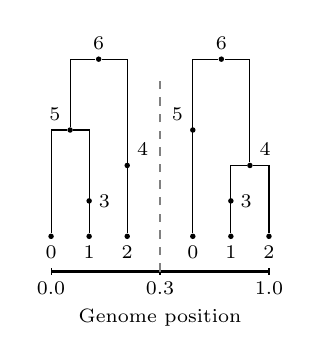
\begin{tikzpicture}[node distance=2mm and 4mm,scale=0.45]

\tikzset{greynode/.style={circle,fill,inner sep=0.7},
nodelabel/.style={font=\scriptsize}}

% Left sample nodes
\node (s0) [greynode] {};
\node (s1) [right=of s0,greynode] {};
\node (s2) [right=of s1,greynode] {};
\foreach \u/\lab in {s0/0, s1/1, s2/2} \node[nodelabel,anchor=north] at (\u) {\lab};

% Right sample nodes
\node (rightTree) at (4, 0) {};
\node [greynode] (s0r) at ($(s0) + (rightTree)$) {};
\node [greynode] (s1r) at ($(s1) + (rightTree)$) {};
\node [greynode] (s2r) at ($(s2) + (rightTree)$) {};
\foreach \u/\lab in {s0r/0, s1r/1, s2r/2} \node[nodelabel,anchor=north] at (\u) {\lab};

% Non-sample nodes
\node [greynode] (s3) at ($(s1) + (0,1)$) {};
\node [greynode] (s3r) at ($(s1r) + (0,1)$) {};
\node [greynode] (s4) at ($(s2) + (0,2)$) {};
\node [greynode] (s4r) at ($0.5*(s1r) + 0.5*(s2r) + (0,2)$) {};
\node [greynode] (s5) at ($0.5*(s0) + 0.5*(s1) + (0,3)$) {};
\node [greynode] (s5r) at ($(s0r) + (0,3)$) {};
\node [greynode] (s6) at ($0.25*(s0) + 0.25*(s1) + 0.5*(s2) + (0,5)$) {};
\node [greynode] (s6r) at ($0.5*(s0r) + 0.25*(s1r) + 0.25*(s2r) + (0,5)$) {};
\foreach \u/\lab in {s3/3, s3r/3} \node[nodelabel,anchor=west] at (\u) {\lab};
\foreach \u/\lab in {s4/4, s4r/4} \node[nodelabel,anchor=south west] at (\u) {\lab};
\foreach \u/\lab in {s5/5, s5r/5} \node[nodelabel,anchor=south east] at (\u) {\lab};
\foreach \u/\lab in {s6/6, s6r/6} \node[nodelabel,anchor=south] at (\u) {\lab};

%% Edges
\foreach \child/\parent in {
	s5/s0, s5/s1, s6/s5, s6/s2,
	s4r/s1r, s4r/s2r, s6r/s0r, s6r/s4r%
}
	\draw (\child) -| (\parent);

% Axes
\draw[very thick] ($(s0) + (0,-1.0)$) -- ($(s2r) + (0,-1.0)$);
\node (topAx) at (0,-1.0) {};
\node (topLeft) at ($(s0) + (0,-1.0)$) {};
\node (genUnit) at ($0.1*(s2r) - 0.1*(s0)$) {};
\foreach \x in {0, 5, 10} \draw ($(topLeft) + \x*(genUnit) + (0,0.1)$) -- +(0, -0.2); % tick marks
\node[anchor=north] at ($(topLeft)$) {\scriptsize 0.0};
\node[anchor=north] at ($(topLeft) + 5*(genUnit)$) {\scriptsize 0.3};
\node[anchor=north] at ($(topLeft) + 10*(genUnit)$) {\scriptsize 1.0};

% Interval endpoints
\draw[thin,color=black!50,dashed] ($(topLeft) + 5*(genUnit)$) -- +(0, 5.5);

% Axis titles
\node (topLabel) at ($(topLeft) + 5*(genUnit) + (0,-1.3)$) {$\scriptsize\textrm{Genome position}$};
\end{tikzpicture}
\end{subfigure}
\begin{subfigure}[t]{0.33\textwidth}
\centering
\caption*{(C)}
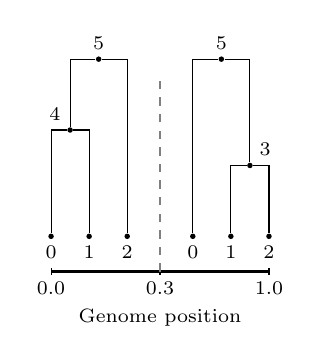
\begin{tikzpicture}[node distance=2mm and 4mm,scale=0.45]

\tikzset{greynode/.style={circle,fill,inner sep=0.7},
nodelabel/.style={font=\scriptsize}}

% Left sample nodes
\node (s0) [greynode] {};
\node (s1) [right=of s0,greynode] {};
\node (s2) [right=of s1,greynode] {};
\foreach \u/\lab in {s0/0, s1/1, s2/2} \node[nodelabel,anchor=north] at (\u) {\lab};

% Right sample nodes
\node (rightTree) at (4, 0) {};
\node [greynode] (s0r) at ($(s0) + (rightTree)$) {};
\node [greynode] (s1r) at ($(s1) + (rightTree)$) {};
\node [greynode] (s2r) at ($(s2) + (rightTree)$) {};
\foreach \u/\lab in {s0r/0, s1r/1, s2r/2} \node[nodelabel,anchor=north] at (\u) {\lab};

% Non-sample nodes
%\node [greynode] (s3) at ($(s1) + (0,1)$) {};
%\node [greynode] (s3r) at ($(s1r) + (0,1)$) {};
%\node [greynode] (s4) at ($(s2) + (0,2)$) {};
\node [greynode] (s4r) at ($0.5*(s1r) + 0.5*(s2r) + (0,2)$) {};
\node [greynode] (s5) at ($0.5*(s0) + 0.5*(s1) + (0,3)$) {};
%\node [greynode] (s5r) at ($(s0r) + (0,3)$) {};
\node [greynode] (s6) at ($0.25*(s0) + 0.25*(s1) + 0.5*(s2) + (0,5)$) {};
\node [greynode] (s6r) at ($0.5*(s0r) + 0.25*(s1r) + 0.25*(s2r) + (0,5)$) {};
%\foreach \u/\lab in {s3/3, s3r/3} \node[nodelabel,anchor=west] at (\u) {\lab};
\foreach \u/\lab in {s4r/3} \node[nodelabel,anchor=south west] at (\u) {\lab};
\foreach \u/\lab in {s5/4} \node[nodelabel,anchor=south east] at (\u) {\lab};
\foreach \u/\lab in {s6/5, s6r/5} \node[nodelabel,anchor=south] at (\u) {\lab};

%% Edges
\foreach \child/\parent in {
	s5/s0, s5/s1, s6/s5, s6/s2,
	s4r/s1r, s4r/s2r, s6r/s0r, s6r/s4r%
}
	\draw (\child) -| (\parent);

% Axes
\draw[very thick] ($(s0) + (0,-1.0)$) -- ($(s2r) + (0,-1.0)$);
\node (topAx) at (0,-1.0) {};
\node (topLeft) at ($(s0) + (0,-1.0)$) {};
\node (genUnit) at ($0.1*(s2r) - 0.1*(s0)$) {};
\foreach \x in {0, 5, 10} \draw ($(topLeft) + \x*(genUnit) + (0,0.1)$) -- +(0, -0.2); % tick marks
\node[anchor=north] at ($(topLeft)$) {\scriptsize 0.0};
\node[anchor=north] at ($(topLeft) + 5*(genUnit)$) {\scriptsize 0.3};
\node[anchor=north] at ($(topLeft) + 10*(genUnit)$) {\scriptsize 1.0};

% Interval endpoints
\draw[thin,color=black!50,dashed] ($(topLeft) + 5*(genUnit)$) -- +(0, 5.5);

% Axis titles
\node (topLabel) at ($(topLeft) + 5*(genUnit) + (0,-1.3)$) {$\scriptsize\textrm{Genome position}$};
\end{tikzpicture}
\end{subfigure}
\caption{\label{fig-arg} (A) A simple ARG in which a recombination
occurs at position 0.3; (B) the equivalent topology depicted as a tree
sequence, including the recombination node; (C) the same tree sequence
topology ``simplified'' down to its minimal tree sequence representation.
Note that the internal nodes have been renumbered in the simplified
representation, so that, e.g., node 5 in (C) corresponds to node 6 in
(A) and (B).}
\end{figure}

For our purposes, an ARG is a realisation of the coalescent with
recombination, in the Griffiths (little ARG) sense.
As described in detail by~\cite{kelleher2016efficient}, Hudson's algorithm
works by dynamically traversing a little ARG.
The graph is not explicitly represented in memory, but is partially
present through the extant lineages and the ancestral material they carry
over time. We do not output the graph directly, but
rather store the information required to recover the genealogical
history as nodes and edges in a tree sequence.
This is far more efficient than outputting the simulated ARG in its entirety.
For a given scaled recombination rate $\rho$
(setting aside the dependency on the sample size $n$)
we know from Eq.~\eqref{eqn-hsw-bound} that the number of nodes
in an ARG is $O(\rho^2)$,
whereas the size of the tree sequence encoding is
$O(\rho)$~\citep{kelleher2016efficient}.
This difference between a
quadratic and a linear dependency on $\rho$ is profound, and shows why
large simulations cannot output an ARG in practice.

Although by default \msprime\ outputs tree sequences that contain full information
about the genealogical trees, their correlation structure along the chromosome,
and the ancestral genomes on which coalescences occurred, some information
is lost in this mapping down from ARG space to the minimal tree sequence
form. In particular, we lose
information about ancestral genomes that were common ancestors but
in which no coalescences occurred, and also information about the precise time
and chromosomal location of recombination events. In most cases, such
information is of little relevance as it is in principle unknowable,
but there are occasions such as visualisation or computing likelihoods (see
below) in which it is useful. We therefore provide
the \texttt{record\_full\_arg} option in \msprime\
to store a representation of the complete ARG traversed during simulation.
This is done by storing extra nodes (marked with specific flags, so they
can be easily identified later) and edges in the tree sequence
(Fig.~\ref{fig-arg}).
One situation in which a record of the full ARG is necessary is when we
wish to compute likelihoods during inference.
The likelihood is a central quantity in evaluating the plausibility of a putative
ancestry as an explanation of DNA sequence data, both directly through
e.g.~approaches based on maximum likelihood, and as an ingredient of
methods such as
Metropolis-Hastings~\citep{kuhner2000maximum,nielsen2000estimation,wang2008bayesian}.
We provide functions to compute the likelihood of ARG realisations
and mutational patterns under
the standard coalescent and infinite sites mutation model.
See the Appendix for details on these likelihood calculations.

\subsection*{Selective sweeps}
\label{sec-selection}
Another elaboration of the standard neutral coalescent with recombination
is the addition of selective
sweeps~\citep{kaplan1989hitchhiking,braverman1995hitchhiking,kim2002detecting}.
Sweeps are modelled by creating a structured population
during the sojourn of the beneficial mutation through the population (i.e., the sweep phase)
in which lineages may transit between favoured and unfavoured backgrounds through
recombination. This allows for many selective sweep scenarios to be simulated
efficiently, including recurrent, partial, and soft selective sweeps.
However in general this
efficiency comes at the cost of flexibility in comparison to forwards in
time simulation.
Several specialised simulators have been developed to simulate
sweeps in the coalescent,
including \texttt{SelSim}~\citep{spencer2004selsim},
\texttt{mbs}~\citep{teshima2009mbs}, \msms~\citep{ewing2010msms},
\cosiTwo~\citep{shlyakhter2014cosi2}
and \discoal~\citep{kern2016discoal}.

\begin{figure}
\begin{center}
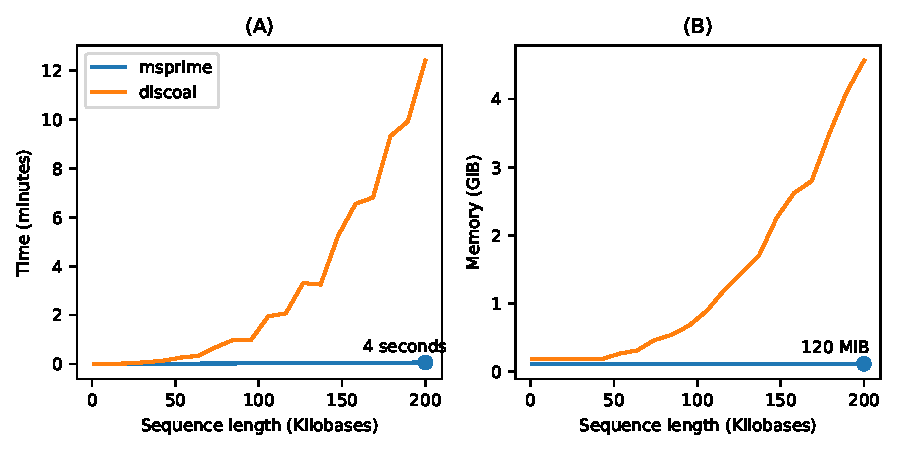
\includegraphics{figures/sweeps-perf}
\end{center}
\caption{\label{fig-selection-perf}Comparison of selective sweep simulation
performance in \msprime\ and \discoal\ (Intel Xeon E5-2680 CPU).
We report the total CPU time and maximum memory usage when simulating 100
replicates for 10 samples in a model
with a single selective sweep in its history where the beneficial
allele had a scaled selection coefficient of $2Ns=1000$,
a per-base recombination rate of $10^{-9}$ and sequence
length varying from 1kb--200kb.}
\end{figure}

Following the approach taken in \discoal, we
have implemented selective sweeps in \msprime\ by generating
sweep trajectories from a jump process approximation to the conditional diffusion
of an allele bound for
fixation~\citep{coop2004ancestral}---see the Appendix for more details.
This implementation facilitates future changes to generalise sweep models to
changing population sizes as well as selection from standing variation.
Moreover because this implements the basic infrastructure for the structured
coalescent, adding support for similar situations,
such as inversions~\citep{peischl2013sequential}, is straightforward.
Fig.~\ref{fig-selection-perf} shows that \msprime\ has far better
CPU time and memory performance than \discoal.

\subsection*{Discrete time Wright-Fisher}
The coalescent is an idealised model and makes many simplifying assumptions,
but it is often surprisingly robust to violations of these
assumptions~\citep{wakeley2012gene}. One situation in which the
model does break down is the combination of large sample size
and long recombining genomes, where the large
number of recombination events in the recent past results in
more than the biologically possible $2^t$ ancestors in
$t$ diploid generations~\citep{nelson2020accounting}.
This pathological behaviour results in
identity-by-descent,
long-range linkage disequilibrium and ancestry patterns deviating from
Wright-Fisher expectations, and the bias grows with larger sample
sizes~\citep{wakeley2012gene,bhaskar2014distortion,nelson2020accounting}.
Precisely this problem occurs when simulating modern human datasets,
and we have implemented a Discrete Time Wright-Fisher (DTWF) model
in \msprime\ to address the issue. The DTWF simulates backwards in
time generation-by-generation so that each gamete has a unique
diploid parent, and multiple recombinations within a generation results in
crossover events between the same two parental haploid copies.
The method is described in more detail by~\cite{nelson2020accounting}.

\begin{figure}
\begin{center}
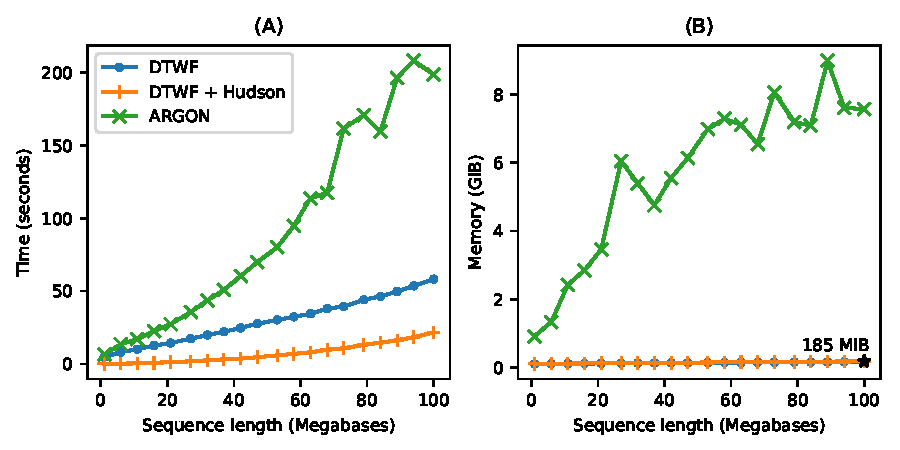
\includegraphics{figures/dtwf-perf}
\end{center}
\caption{\label{fig-dtwf-perf} Comparison of Discrete Time Wright-Fisher
(DTWF) simulation performance in \msprime\ and \ARGON\ (Intel Xeon E5-2680 CPU).
We simulated ancestry for a sample of 1000 haploids from a population of 10000,
and report the (A) total CPU time and (B) maximum memory usage for varying
sequence lengths, and a per-base recombination rate of $10^{-8}$. Each
point is the average over $5$ replicate simulations.
We show observations for \ARGON, \msprime's DTWF implementation (``DWTF'')
and a hybrid simulation of 100 generations of the DTWF followed by
the standard coalescent with recombination model (``DTWF + Hudson'').
Memory usage for \msprime's DTWF and hybrid simulations are very similar.
We ran \ARGON\ with a mutation rate of $0$ and with minimum output options,
to ensure we are measuring only ancestry simulation time.}
\end{figure}

Fig.~\ref{fig-dtwf-perf} shows that \msprime\ simulates the DTWF
more quickly and requires substantially less memory than
\ARGON~\citep{palamara2016argon}, a specialised DTWF simulator.
However, the generation-by-generation approach of the DTWF is less
efficient than the coalescent with recombination when the
number of lineages is significantly less than the population size
(the regime where the coalescent is an accurate approximation),
which usually happens in the quite recent
past~\citep{bhaskar2014distortion}.
We therefore support changing the simulation model during a simulation
so that we can run hybrid simulations, as proposed by~\cite{bhaskar2014distortion}.
Any number of different simulation models can be combined, allowing for the
flexible choice of simulation scenarios.
As the discrete time Wright-Fisher model improves accuracy of genealogical
patterns in the recent past, we can simulate the recent history using this
model and then switch to the standard coalescent to more efficiently simulate
the more ancient history.

\subsection*{Integration with forward simulators}
A unique feature of \msprime\ is its ability to simulate
genetic ancestries by extending an existing partial
genetic ancestry. Given a tree sequence that
is complete up until time $t$ ago as input
(where marginal trees may or may not have fully coalesced),
\msprime\ can efficiently obtain the segments of ancestral material
present at this time, and then run the simulation backwards in time from there.
This allows a simulated ancestry to be produced by any
number of different processes across disjoint time slices.
In practice this feature is used to ``complete''
forwards-time ancestry simulations~\citep{kelleher2018efficient}
that may have not fully coalesced. This process
(``recapitation'') can be orders of magnitude faster than
the standard approach of neutral burn-in; see
\cite{haller2018tree} for more details and examples.
This interoperability between simulators, where a partial ancestry
simulation produced by \SLiM~\citep{haller2019slim}
or \fwdpy~\citep{thornton2014cpp} can be picked up and completed
by another simulator, with complete information
retained---at scale---is unprecedented.
This interoperability indicates an opportunity for
other forward genetic simulators ~\citep[e.g.][]{Gaynor2021AlphaSimR}
to leverage the tree sequence data format and associated tools.

\subsection*{Development model}
\texttt{Msprime} has a large number of features, encompassing
the functionality of several more specialised simulators
while maintaining excellent performance.
It is developed by a geographically distributed team of volunteers under an
open source community development model, with a strong emphasis
on code quality, correctness, good documentation, and inclusive development.
As in any large code base,
unit tests play a key role in ensuring that new additions behave
as expected and \msprime\ has an extensive suite.
As of the 1.0.0 release \msprime\ consists of around 13K lines of C and 11K
lines of Python, with suites of 122 C tests (7K lines of code) and
1350 Python tests (22K lines of code). These tests are run
automatically on different operating systems on each pull request
(where a contributor proposes a code change), using standard Continuous
Integration (CI) methodology. Other CI services
check for common errors, code formatting issues, and produce reports on
the level of test coverage for the proposed change.

Unit tests are vital for ensuring software quality and correctness, but
they are usually of little value in assessing the statistical properties
of simulations. To validate the correctness of simulation output
we maintain a suite of statistical tests (as of 1.0.0,
217 validation tests, in 6K lines of code). These consist of running many
replicate simulations to check the properties of the output
against other simulators, and where possible against analytical results.
For example, simulations of complex demography are validated against \ms,
selective sweeps against \discoal, and Wright-Fisher simulations
against forwards in time simulations in \SLiM.
This suite of tests is run before every release, to ensure
that statistical errors have not been introduced.

More visibly to the end user, we also have a high standard for documentation,
with precise, comprehensive, and cross-linked documentation
that is automatically built from the code base
and served through the website \texttt{https://tskit.dev}.
With the goal of lowering the entry barrier to new users,
we have invested significant effort in writing examples and introductions,
and making common tasks discoverable.
We also view contributions to documentation as equally important to the project
as writing code or designing methods: what use would it be
to write reliable, stable software if no-one used it?

\section*{Discussion}

% We can simulate so much more now
The 1.0 release of \msprime\ marks a major increase in the
breadth of available features and the
potential biological realism of simulations.
These abilities will allow researchers to perform more robust power analyses,
more reliably test new methods,
carry out more reliable inferences,
and more throughly explore the properties of theoretical models.
Despite this complexity and generality,
\msprime's performance is state-of-the-art
and all features are thoroughly tested and statistically validated.
These advances have only been possible thanks to a distributed,
collaborative model of software development,
and the work of many people.
% We hope the tool continues to be useful to many.

% Simulation software is historically a beautiful shitshow

Even though simulation has long been a vital tool in population genetics,
such collaborative software development has historically been uncommon.
A huge proliferation of tools have been published
(the references here are not exhaustive)
and only a small minority of these are actively developed and
maintained today. The ecosystem is highly fragmented, with numerous different
ways of specifying parameters and representing results, and there are
significant software quality issues at all stages. This is unsurprising, since
the majority of simulation software development is performed by students,
often without formal training in software development.
Although this ``Haldane's sieve'' of software has produced many good tools
and enabled decades of research,
it also represents a missed opportunity to invest as a community
in shared infrastructure and mentorship in good software development practice.

% THERE IS A BETTER WAY!!!
Scientific software is vital apparatus, and must be engineered
to a high quality if we are to trust its results. There is a growing
realisation across the sciences
% More citations?
\citep[e.g.][]{siepel2019challenges,harris2020array,gardner2021sustained}
that investing in
shared community infrastructure produces better results than a
proliferation of individually maintained tools, allowing scientists
to focus on their specific questions rather than software engineering.
\texttt{Msprime} 1.0 is the result of such a community process,
with features added by motivated users, taking advantage of the
established development practices and infrastructure.
Software development in a welcoming community,
with mentorship by experienced developers,
is a useful experience for many users.
The skills that contributors learn
can lead to greatly increased productivity in subsequent
work (e.g., through more reliable code and better debugging skills).
We hope that users who find that
features they require are missing will continue to contribute to
\msprime, leading to a community project that is both high quality
and sustainable in the long term.

The succinct tree sequence data structure developed
for \msprime\ provides a view of not only
genetic variation, but also the genetic ancestry that produced that variation.
Recent breakthroughs in methods to infer genetic ancestry in recombining
organisms~\citep{rasmussen2014genome,kelleher2019inferring,
speidel2019method,wohns2021unified,schaefer2021ancestral,speidel2021inferring}
have made it possible to estimate such ancestry from real data at scale for
the first time~\citep{harris2019database,tang2019genealogy}.
Given such inferred ancestry, many exciting applications
become possible. For example, \cite{osmond2021estimating}
developed a method to estimate the location of genetic ancestors
based on inferred trees, and other uses are sure to follow.
Since the inferred genetic ancestry
becomes the input for other downstream inferences, it is vitally
important that these primary inferences are thoroughly validated,
with the detailed properties of the inferred ancestries
catalogued and understood.
\texttt{Msprime} will continue to be an important tool for these inferences and validations,
and in this context the ability to interoperate
with other methods---particularly forwards simulators---through
the succinct tree sequence data structure and \tskit\ library
will be essential.
% this final sentence is hard to parse

\section*{Acknowledgements}
We would like to thank Iain Mathieson and Alywyn Scally for helpful comments
on the manuscript.
% alphabetised by author. Names spelled out if there's an initial collision
ADK was supported by NIH awards R01GM117241 and R01HG010774.
BE was supported by  DFG grant  273887127 through Priority Programme SPP 1819: Rapid Evolutionary Adaptation (grant STE 325/17-2) to Wolfgang Stephan; BE would also like to acknowledge  funding through The Icelandic Research Centre (Rann{\'i}s) through an Icelandic Research Fund Grant of  Excellence nr.\ 185151-051 to Einar \'Arnason,  Katr\'in Halld\'orsd\'ottir,  Alison Etheridge,  Wolfgang Stephan, and BE.
FB is funded by the Deutsche Forschungsgemeinschaft EXC 2064/1 -- Project number 390727645, and EXC 2124 -- Project number 390838134.
Graham Gower was supported by a Villum Fonden Young Investigator award to Fernando Racimo (project no. 00025300).
Gregor Gorjanc is supported by the Chancellor's Fellowship of the University of Edinburgh and the BBSRC grant to The Roslin Institute BBS/E/D/30002275.
Jere Koskela is supported in part by EPSRC grant EP/R044732/1.
Jerome Kelleher is supported by the Robertson Foundation.
SG acknowledges funding from the Canada Research Chairs Program, from the Canadian Institutes of Health Research PJT 173300, and from the Canadian Foundation for Innovation.

\bibliographystyle{plainnat}
\bibliography{paper}


%% local definitions for section multiple merger coalescents
 \newcommand{\be}{\begin{equation}}
 \newcommand{\ee}{\end{equation}}
 \newcommand{\bd}{\begin{displaymath}}
 \newcommand{\ed}{\end{displaymath}}
\newcommand{\IN}{\ensuremath{\mathds{N}}}%
\newcommand{\EE}[1]{\ensuremath{\mathds{E}\left[ #1 \right]}}%
\newcommand{\one}[1]{\ensuremath{\mathds{1}_{\left\{ #1 \right\}}}}%
\newcommand{\prb}[1]{\ensuremath{\mathds{P}\left( #1 \right) } }%

\NewEnviron{esplit}[1]{%
\begin{equation}
\label{#1}
\begin{split}
  \BODY
\end{split}\end{equation}
}

\setcounter{secnumdepth}{2} % Print out appendix section numbers

\appendix
\section*{Appendix}

\subsection*{Mutation generation}
\label{app-mutation-algorithm}

The algorithm that \msprime\ uses to simulate mutations on a tree sequence
proceeds in two steps:
first, mutations are ``placed'' on the tree sequence
(i.e., sampling their locations in time, along the genome, and on the marginal tree),
and then the ancestral and derived alleles of each mutation are generated.
All mutation models share the code to place mutations,
but choose alleles in different ways.

First, mutations are placed on the tree sequence under an inhomogeneous Poisson model
by applying them independently to each edge.
If an edge spans a region $[a, b)$ of the genome
and connected parent and child nodes with times $s < t$,
and the mutation rate locally is $\mu$,
then the number of mutations on the edge is Poisson with mean $\mu (t-s) (b-a)$,
and each mutation is placed independently at a position chosen uniformly in $[a,b)$
and a time uniformly in $[s,t)$.
In a discrete genome, all positions are integers and so more than one mutation
may occur at the same position on the same edge.
Otherwise (i.e., for an infinite-sites model),
positions are rejection sampled to obtain a unique floating-point number.
If an edge spans a region of the genome with more than one mutation rate,
this is done separately for each sub-region on which the mutation rate is constant.
Since each edge is processed independently, the algorithm
scales linearly with the number of edges in the tree sequence.

Next, alleles are chosen for each mutation.
If the site was not previously mutated, then a new ancestral allele is chosen for the site,
according to an input distribution of ancestral state allele probabilities.
Then, each mutation on the tree is considered in turn,
and a derived allele is randomly chosen based on the parental allele
(which may be the ancestral allele or the derived allele of a previous mutation).
Finally, information about the mutations are recorded in the site and mutation tables
of the tree sequence.

A mutation model must, therefore, provide two things:
a way of choosing an ancestral allele for each new variant site,
and a way of choosing a derived allele given the parental allele at each mutation.
Perhaps the simplest mutation model implemented in \msprime\ is the
\texttt{InfiniteAlleles} mutation model,
which keeps an internal counter so that the requested alleles are
assigned subsequent (and therefore unique) integers.

The distribution of ancestral alleles
is used to choose the allele present at the root of the tree at each mutated site,
i.e., the \texttt{root\_distribution}.
Mutation models with a finite possible set of alleles have a natural choice
for this distribution---the \emph{stationary distribution} of the mutation process.
(All mutation models are Markovian,
so this may be found as the top left eigenvector of the mutation matrix.)
This is the default in most models,
except, e.g., the \texttt{BinaryMutationModel}, whose alleles are 0 and 1
and always labels the ancestral allele ``0''.
However, mutational processes are not in general stationary,
so we often allow different root distribution to be specified.

Since the general algorithm above applies mutations at a single rate
independent of ancestral state,
a model in which different alleles mutate at different rates
must necessarily produce some silent mutations,
i.e., mutations in which the derived allele is equal to the parental allele.
To illustrate this, consider a mutation model
in which $A$ or $T$ mutates to a randomly chosen different nucleotide at rate $\alpha$
and $C$ or $G$ mutates at rate $\beta$, with $\beta < \alpha$.
To implement this, first place mutations at the largest total rate, which is $\alpha$.
Then, at each site, choose an ancestral allele from the root distribution,
and for each mutation, choose a derived allele as follows:
if the parental allele is $A$ or $T$, then choose a random derived allele
different to the parental allele;
if the parental allele is $C$ or $G$,
then choose the derived allele to be equal to the parent allele
with probability $\beta/(\alpha + \beta)$,
and randomly choose a different nucleotide otherwise.
This produces the correct distribution by Poisson thinning:
a Poisson process with rate $\alpha$ in which each point is discarded independently
with probability $\beta / (\alpha + \beta)$ is equivalent to a Poisson
process with rate $\beta$.
All finite-state models (implemented under the generic \texttt{MatrixMutationModel} class)
work in this way: mutations are placed at the maximum mutation rate,
and then some silent mutations will result.

In previous versions of \msprime, silent mutations were disallowed,
and we could have removed them from the output entirely.
However, we have chosen to leave them in, so that for instance
simulating with the \texttt{HKY} mutation model will result in silent mutations
if not all equilibrium frequencies are the same.
The presence of silent mutations may at first be surprising
(although they are fully accounted for in downstream calculations of statistics
by \tskit),
but there is a good reason to leave them in:
to allow layering of different mutation models.
Suppose that we wanted to model the mutation process as a mixture of more than one model,
e.g., Jukes-Cantor mutations at rate $\mu_1$, and
HKY mutations occur at rate $\mu_2$.
Layering multiple calls to \texttt{sim\_mutations} is allowed,
so we could first apply mutations with the \texttt{JC69} model at rate $\mu_1$
and then add more with the \texttt{HKY} model at rate $\mu_2$.
However, there is a small statistical problem:
suppose that after applying Jukes-Cantor mutations we have an $A \to C$ mutation,
but then the HKY mutations inserts another mutation in the middle,
resulting in $A \to C \to C$.
If neither mutation model allows silent transitions,
then this is clearly not correct,
i.e., it is not equivalent to a model that simultaneously applies the two models.
(The impact is small, however, as it only affects sites with more than one mutation.)
The solution is to make the Jukes-Cantor model \emph{state-independent}
(also called ``parent-independent''),
by placing mutations at rate $4/3 \mu_1$ and then choosing the derived state for each mutation
\emph{independently} of the parent (so that 1/4 of mutations will be silent).
If so---and, more generally, if the first mutational process put down is
state-independent---then the result of sequentially applying the two mutation models
is equivalent to the simultaneous model.
To facilitate this, many mutation models have a \texttt{state\_independent} option
that increases the number of silent mutations
and makes the model closer to state-independent.


\subsection*{Likelihood calculations}
\label{app-likelihoods}

We provide two functions to facilitate likelihood-based inference.
Both are implemented only for the simplest case of the standard ARG with a
constant population size, and require tree sequences compatible with the
\texttt{record\_full\_arg} option as their arguments.

The \texttt{msprime.log\_arg\_likelihood(ts, r, N)} function
returns the natural logarithm of
the sampling probability of the tree sequence \texttt{ts} under the ARG with per-link,
per-generation recombination probability \texttt{r} and population size \texttt{N}.
Specifically, the function returns the logarithm of
\begin{equation*}
\Bigg( \frac{ 1 }{ 2 N } \Bigg)^{ q_c } \Bigg( \prod_{ i : \mathcal{R} } r g_i \Bigg)
	\exp\Bigg( -\sum_{ i = 1 }^q \Big[\frac{ 1 }{ 2 N } \binom{ k_i }{ 2 }
		+ r l_i \Big] t_i  \Bigg),
\end{equation*}
where $t_i$ is the number of generations between the $(i - 1)$th and $i$th event,
$k_i$ is the number of extant ancestors in that interval, $l_i$ is the number of links
in that interval that would split ancestral material should they recombine,
$q$ is the total number of events in the tree sequence $\texttt{ts}$,
$q_c$ is the number of coalescences, $\mathcal{R}$ is the set of indices
of time intervals which end in a recombination, and $g_i$ is the corresponding
\emph{gap}:  the length of material in which the recombination at the end of the
$i$th period could have taken place without affecting the resulting genealogy.
A recombination in ancestral material will always have $g_i = 1$, while a recombination
in trapped non-ancestral material can result in other values of $g_i$.
For a continuous model of the genome and a recombination in ancestral material,
we set $g_i = 1$ and interpret the result as a density.

The \texttt{msprime.unnormalised\_log\_mutation\_likelihood(ts, m)} function returns the
natural logarithm of the probability of the mutations recorded in the tree sequence
\texttt{ts} given the corresponding ancestry, assuming the infinite sites model, up to
a normalising constant which depends on the pattern of mutations,
but not on the tree sequence or the per-site, per-generation mutation
probability \texttt{m}.
Specifically, the function returns the logarithm of
\begin{equation*}
e^{ - T m / 2 } \frac{ ( T m / 2 )^M }{ M ! }
\prod_{ \gamma \in \mathcal{ M } } \frac{ h_{ \gamma } }{ T },
\end{equation*}
where $T$ and $\mathcal{M}$ are the total branch length and set of mutations
in \texttt{ts}, respectively, and for a mutation $\gamma$, $h_{ \gamma }$ is the
total branch length on which $\gamma$ could have arisen while appearing on all
of the leaves of \texttt{ts} it does, and on no others.
Unary nodes on marginal trees arising from the \texttt{record\_full\_arg} option
mean that, in general $h_{ \gamma }$ corresponds to the length of one or more
edges.
% \end{itemize}


\label{app-multiple-mergers}
\subsection*{Multiple merger coalescent model}

Multiple merger coalescents, in which a random number of ancestral
lineages may merge into a common ancestor at a given time,
are referred to as $\Lambda$-coalescents.
The rate at which  a given group of $k$ out of a total of  $b$ lineages merges  is
\begin{equation}\label{lambdabk}
\lambda_{b, k} =  \int_0^1  x^{k-2}(1-x)^{b-k}\Lambda(dx) + a\one{k=2}, \quad 2 \le k \le b,
\end{equation}
where $a \geq 0$ is a constant and $\Lambda$ is a finite measure on the unit interval without an atom at zero \citep{DK99,P99,S99}.
There is also a larger class of simultaneous multiple merger coalescents involving
simultaneous mergers of distinct groups of lineages into several common ancestors \citep{S00}.
These are commonly referred to as $\Xi$-coalescents, and
often arise from population models incorporating diploidy or more general polyploidy
\citep{BBE13,blath2016site}.
To describe a general $\Xi$-coalescent, let $\Delta$ denote the
infinite simplex
\begin{equation*}
 \Delta := \Bigg\{ (x_1,x_2,  \ldots ): x_1 \ge x_2 \ge \cdots \ge 0, \sum_{j = 1}^{ \infty} x_j \le 1\Bigg\}.
 \end{equation*}
The rate of mergers is determined by
$\Xi = \Xi_0 + a\delta_0$, where $a \geq 0$ is a constant, $\delta_0$ is the Dirac delta
measure, and $\Xi_0$ is a finite measure on $\Delta$ with no atom at (0, 0, \ldots).
For an initial number of blocks $b \geq 2$ and
$r \in \{1,2, \ldots, b - 1 \}$, let $k_1 \geq 2, \ldots, k_r \ge 2$ be the sizes of $r$ merger events
and $s = b - k_1 - \cdots - k_r$ be the number of blocks not participating in any merger.
The rate of each possible set of mergers with sizes $(k_1, \ldots, k_r)$ is
\begin{align*}
  \lambda_{n; k_1, \ldots, k_r; s}  = {}& \int_\Delta  \sum_{\ell = 0}^s \sum_{\substack {i_1, \ldots, i_{r+\ell} = 1\\ \text{all distinct}} }^\infty  \binom{s}{\ell} x_{i_1}^{k_1} \cdots  x
_{i_{r}}^{k_r} x_{i_{r+1}} \cdots x_{i_{r+\ell}}\left(1 - \sum_{j=1}^\infty x_j \right)^{s-\ell} \frac{1}{ \sum_{j=1}^\infty x_j^2 } \Xi_0(dx)   \\
  & +  a\one{r=1, k_1 = 2},
\end{align*}
and the number of such $(k_1, \ldots, k_r)$ mergers is
\begin{equation*}
    \mathcal{N}(b; k_1, \ldots, k_r ) = \binom{b}{k_1 \ldots k_r\, s} \frac{1}{ \prod_{j=2}^b\ell_j!  },
\end{equation*}
where $\ell_j := \#\{ i \in \{ 1, \ldots, r \} : k_i = j \}$ is the number of mergers of size $j \geq 2$ \citep{S00}.

Viewing coalescent processes strictly as mathematical
objects, it is clear that the class of $\Xi$-coalescents contains
$\Lambda$-coalescents as a specific example in which at most
one group of lineages can merge at each time, and the class of
$\Lambda$-coalescents contain the Kingman-coalescent as a special
case.  However, viewed as limits of ancestral processes derived from
specific population models they are not nested. For example, one can
obtain $\Lambda$-coalescents from haploid population models
incorporating sweepstakes reproduction and high fecundity,
and $\Xi$-coalescents for the same models for diploid populations \citep{BBE13}.
One should therefore apply the models as appropriate, i.e.\
$\Lambda$-coalescents to haploid (e.g.\ mtDNA) data,
and $\Xi$-coalescents to diploid or polyploid (e.g.\ autosomal) data \citep{blath2016site}.


In \msprime\ we have incorporated two examples of multiple-merger coalescents.
One is a diploid extension \citep{BBE13} of the haploid Moran model adapted
to sweepstakes reproduction considered by \cite{EW06}.
Let $N$ denote the population size, and take $\psi \in (0,1]$ to be fixed.
In every generation, with probability $1-\varepsilon_N$ a single individual
(picked uniformly at random) perishes.
With probability $\varepsilon_N$, $\lfloor \psi N \rfloor$ individuals picked uniformly
without replacement perish instead.
In either case, a surviving individual picked uniformly at random produces enough offspring
to restore the population size back to $N$.  Taking $\varepsilon_N =
1/N^\gamma$ for some $\gamma > 0$, \cite{EW06} obtain $\Lambda$-coalescents
for which the $\Lambda$ measure in \eqref{lambdabk} is a
point mass at $\psi$.  The simplicity of this model does allow one to obtain
some explicit mathematical results (see e.g.\
\cite{Der2012, EF2018,Freund2020,Matuszewski2017}), and the model has also been
used to simulate gene genealogies within phylogenies \citep{zhu2015hybrid}.
As well as the haploid model of \cite{EW06}, \msprime\ provides the diploid version
of \cite{BBE13}, in which individuals perish as above, but replacements are
generated by sampling a single pair of diploid individuals as parents, with
children sampling one chromosome from each parent.
Hence, there are four parent chromosomes involved in each reproduction event, which can lead to
up to four simultaneous mergers, giving rise to a $\Xi$-coalescent with merger rate
\begin{esplit}{Cconst} \lambda^{\text{Dirac}}_{b; k_1, \ldots,
k_r;s } &= \frac{c \psi^2 / 4}{1 + c \psi^2 / 4} \frac{4}{ \psi^2}\sum_{\ell = 0}^{s \wedge (4-r)} \binom{s}{\ell}
(4)_{r+\ell} (1-\psi)^{s-\ell }\left( \frac{\psi}{4} \right) ^{k_1 + \cdots +
k_r + \ell} + \frac{\one{r=1, k_1 = 2}}{1 + c \psi^2 / 4},  \\ \end{esplit}
The interpretation of \eqref{Cconst} is that `small' reproduction events in which
two lineages merge occur at rate $1/(1 + c\psi^2/4)$, while large reproduction events
with the potential to result in simultaneous multiple mergers occur at rate $(c\psi^2/4) / (1 + c\psi^2/4)$.


The other multiple merger coalescent model incorporated in \msprime\ is
the haploid population model considered by \cite{schweinsberg03},
as well as its diploid extension \citep{BLS15}.  In the haploid
version, in each generation of fixed size $N$, individuals produce random numbers of
juveniles $(X_1, \ldots, X_N)$ independently, each distributed according to a stable law satisfying
\be\label{jX} \lim_{k\to \infty} C k^\alpha \prb{X \ge k} = 1 \ee
with index $\alpha > 0$, and where $C > 0$ is a normalising constant.
If the  total number of juveniles $S_N := X_1 + \ldots + X_N$ produced
in this way is at least $N$, then $N$ juveniles are sampled uniformly at random
without replacement to form the next generation.
As long as $\EE{X_1} > 1$, one can show that $\{ S_N < N \}$ has exponentially small
probability in $N$, and does not affect the resulting coalescent as $N \to \infty$ \citep{schweinsberg03}.
If $\alpha \ge 2$ the ancestral process converges to the Kingman-coalescent; if
$1 \le \alpha < 2$ the ancestral process converges to a $\Lambda$-coalescent
with $\Lambda$ in \eqref{lambdabk} given by the Beta$(2-\alpha, \alpha)$ distribution, i.e.\
\be\label{Fbeta} \Lambda(dx) = \one{0< x \le 1} \frac{1}{B(2-\alpha,\alpha)}
x^{1 - \alpha}(1-x)^{\alpha - 1}  dx, \ee where
$B(a,b) = \Gamma(a)\Gamma(b)/\Gamma(a+b)$ for $a,b > 0$ is the
beta function \citep{schweinsberg03}.
This model has been adapted to diploid populations
by \cite{BLS15}, and the resulting coalescent is $\Xi$-coalescent with merger rate
\be\label{xibeta} \lambda_{b;k_1, \ldots, k_r; s}^{\text{Beta}} = \sum_{\ell = 0}^{ s\wedge (4-r) } \binom{s}{\ell} \frac{ (4)_{r+\ell} }{4^{k+\ell}}
\frac{B(k+\ell - \alpha, s-\ell + \alpha ) }{B(2-\alpha,\alpha)}, \ee
where $k := k_1 + \ldots + k_r$ \citep{blath2016site,BLS15}. The interpretation of \eqref{xibeta} is  that the
random number of lineages participating in a potential merger is governed by the
$\Lambda$-coalescent with rate \eqref{Fbeta}, and all participating lineages are
randomly allocated into one of four groups corresponding to the four parental
chromosomes, giving rise to up to four simultaneous mergers.

The stable law \eqref{jX} assumes that individuals can produce arbitrarily
large numbers of juveniles. Since juveniles are at least fertilised eggs,
it may be desirable to suppose that the number of juveniles
surviving to reproductive maturity cannot be arbitrarily large.  Hence we also consider
an adaptation of the \cite{schweinsberg03} model, where
the random number of juveniles has a deterministic upper bound $\phi(N)$,
and the distribution of the number of juveniles produced by a given parent
(or pair of parents in the diploid case) is
\be\label{jtr} \prb{X=k} =   \one{1 \le k \le \phi(N)}
\frac{\phi(N+1)^\alpha }{ \phi(N+1)^\alpha - 1 }  \left( \frac{1}{k^\alpha} -
\frac{1}{(k+1)^\alpha}  \right) . \ee
See \citet{Eldon2018} for a related model.   One can follow the calculations of
\cite{schweinsberg03} or \cite{BLS15}  to show  that  if $1 < \alpha < 2$
then, recalling that $k = k_1 + \cdots + k_r$, the merger rate is
 \be \lambda_{b;k_1, \ldots, k_r; s}^{\text{Beta}, M} =  \sum_{\ell = 0}^{ s \wedge (4-r) }
\binom{s}{\ell} \frac{ (4)_{r+\ell} }{4^{k+\ell}} \frac{B(M; k+\ell - \alpha,
s-\ell + \alpha ) }{B(M;2-\alpha,\alpha)}
\ee
where $B(z;a,b) := \int_0^z
t^{a-1}(1-t)^{b-1}dt$ for  $a,b>0$ and $0< z\le 1$ is the incomplete beta function, and
\begin{equation*}
M :=  \lim_{ N \to \infty } \frac{\phi(N) / N}{\phi(N) / N + \EE{X_1}} \in (0, 1]
\end{equation*}
\citep{CDEE2020}.    In other words,  the measure $\Lambda$ driving
the multiple mergers is of the same form as in \eqref{Fbeta}  with $0 < x
\le M$ in the case $1 < \alpha < 2$ and $\lim_{ N \to \infty } \phi(N) / N > 0$.   If $\alpha \ge 2$
or $\phi(N)/N \to 0$ then  the  ancestral process converges to  the Kingman-coalescent
\citep{CDEE2020}.

\label{app-sweeps}
\subsection*{Selective sweep trajectories}
We have implemented the coalescent with selective sweeps as a structured
coalescent process (as in~\citep{braverman1995hitchhiking}). During the
``sweep phase'' of the simulation the rate of coalescence and recombination
is tracked separately in lineages linked to the beneficial allele or not,
with those rates depending on the frequency of the beneficial allele in
the population at a given time. The allele frequency trajectory of the
sweeping allele is modelled using a jump process that approximates
the conditional diffusion of the allele, conditioning on its eventual
fixation~\citep{coop2004ancestral}.
The jump process moves back in time following the beneficial
allele frequency, $p$, from some initial frequency (e.g., $p=1$) back to
the origination of the allele at $p=1/2N$, and we track time in small
increments $\delta t$. This works such that the allele frequency at
the next time step back in time, call it $p^\prime$ is

\begin{eqnarray*}
	p'=\left\{ \begin{array}{ll}
	    p + \mu(p)\delta t +\sqrt{p(1-p)\delta t} & \quad \mbox{with probability $1/2$}\\
	    p + \mu(p)\delta t -\sqrt{p(1-p)\delta t} & \quad \mbox{with probability $1/2$}\\
	\end{array} \right.
\end{eqnarray*}
where
\begin{eqnarray*}
	\mu(p)=\frac{\alpha p (1 - p)}{tanh(\alpha(1-p))}.
\end{eqnarray*}
Here, $\alpha=2Ns$ and $s$ is the fitness advantage in homozygotes. This model
assumes genic selection (i.e., that the dominance coefficient $h=0.5$).

While our current implementation only deals with genic selection,
we plan in the future to add sweeps with arbitrary dominance. Further planned
additions include trajectories of purely neutral alleles, as well as trajectories
that model soft selective sweeps.



\end{document}
